% The command below calls the preprint style^M
% which will produce a one-column, single-spaced document.^M
% Examples of commands for other sub-styles follow. Use^M
% whichever is most appropriate for your purposes.^M

%\documentclass[12pt,preprint]{aastex}
%\documentclass[iop,appendixfloats]{emulateapj}

% manuscript produces a one-column, double-spaced document:

%\documentclass[manuscript]{aastex}
%----------------------------------
% mn2esample.tex
%
% v2.1 released 22nd May 2002 (G. Hutton)
%
% The mnsample.tex file has been amended to highlight
% the proper use of LaTeX2e code with the class file
% and using natbib cross-referencing. These changes
% do not reflect the original paper by A. V. Raveendran.
%
% Previous versions of this sample document were
% compatible with the LaTeX 2.09 style file mn.sty
% v1.2 released 5th September 1994 (M. Reed)
% v1.1 released 18th July 1994
% v1.0 released 28th January 1994

\documentclass[useAMS,usenatbib,letters]{mn2e}

% If your system does not have the AMS fonts version 2.0 installed, then
% remove the useAMS option.
%
% useAMS allows you to obtain upright Greek characters.
% e.g. \umu, \upi etc.  See the section on "Upright Greek characters" in
% this guide for further information.
%
% If you are using AMS 2.0 fonts, bold math letters/symbols are available
% at a larger range of sizes for NFSS release 1 and 2 (using \boldmath or
% preferably \bmath).
%
% The usenatbib command allows the use of Patrick Daly's natbib.sty for
% cross-referencing.
%
% If you wish to typeset the paper in Times font (if you do not have the
% PostScript Type 1 Computer Modern fonts you will need to do this to get
% smoother fonts in a PDF file) then uncomment the next line
% \usepackage{Times}

%%%%% AUTHORS - PLACE YOUR OWN MACROS HERE %%%%%
\usepackage{color}
\usepackage{graphicx}
\usepackage{amsmath}
\usepackage{amssymb}
\definecolor{orange}{rgb}{1,0.5,0}
\usepackage[colorlinks=True,citecolor=orange,urlcolor=blue,linkcolor=red]{hyperref}

\newcommand{\figurepath}{.}


%  Definition of fonts


\newcommand{\tom}{\tilde{\omega}}

\newcommand{\ri}{r_{\rm i}}

\newcommand{\ro}{r_{\rm out}}

\newcommand{\rs}{r_{\star}}

\newcommand{\mj}{\dot{M}_{\rm jet}}

\newcommand{\ms}{\dot{M}_{\star}}

\newcommand{\vk}{v_{\rm K}}

\newcommand{\ti}{t_{\rm i}}

\newcommand{\rj}{R_{\rm jet}}

\newcommand{\rk}{R_{\kappa}}

\newcommand{\cs}{c_{\rm s}}

\newcommand{\css}{c_{\rm s}^2}

\newcommand{\bp}{B_{\rm P}}

\newcommand{\bh}{B_{\phi}}

\newcommand{\jp}{\vec{B}_{\rm P}}

\newcommand{\cm}{{\rm cm}}

\newcommand{\msun}{{\rm M}_{\sun}}

\newcommand{\rsun}{{\rm R}_{\sun}}

\newcommand{\rstar}{{\rm R}_{\star}}

\newcommand{\lumsun}{{\rm L}_{\sun}}

\newcommand{\lumstar}{{\rm L}_{\star}}

\newcommand{\lumdisk}{{\rm L}_{\rm disk}}

\newcommand{\etat}{{\eta}_{\rm t}}

\newcommand{\betat}{{\beta}_{\rm t}}

\newcommand{\betai}{{\beta}_{\rm i}}

\newcommand{\deltai}{{\delta}_{\rm i}}

\newcommand{\rhoi}{{\rho}_{\rm i}}
\newcommand{\refer}{{\color{orange}REFERENCE}}

% Bibliography and bibfile
\def\aj{AJ}%
          % Astronomical Journal
\def\actaa{Acta Astron.}%
          % Acta Astronomica
\def\araa{ARA\&A}%
          % Annual Review of Astron and Astrophys
\def\apj{ApJ}%
          % Astrophysical Journal
\def\apjl{ApJ}%
          % Astrophysical Journal, Letters
\def\apjs{ApJS}%
          % Astrophysical Journal, Supplement
\def\ao{Appl.~Opt.}%
          % Applied Optics
\def\apss{Ap\&SS}%
          % Astrophysics and Space Science
\def\aap{A\&A}%
          % Astronomy and Astrophysics
\def\aapr{A\&A~Rev.}%
          % Astronomy and Astrophysics Reviews
\def\aaps{A\&AS}%
          % Astronomy and Astrophysics, Supplement
\def\azh{AZh}%
          % Astronomicheskii Zhurnal
\def\baas{BAAS}%
          % Bulletin of the AAS
\def\bac{Bull. astr. Inst. Czechosl.}%
          % Bulletin of the Astronomical Institutes of Czechoslovakia 
\def\caa{Chinese Astron. Astrophys.}%
          % Chinese Astronomy and Astrophysics
\def\cjaa{Chinese J. Astron. Astrophys.}%
          % Chinese Journal of Astronomy and Astrophysics
\def\icarus{Icarus}%
          % Icarus
\def\jcap{J. Cosmology Astropart. Phys.}%
          % Journal of Cosmology and Astroparticle Physics
\def\jrasc{JRASC}%
          % Journal of the RAS of Canada
\def\mnras{MNRAS}%
          % Monthly Notices of the RAS
\def\memras{MmRAS}%
          % Memoirs of the RAS
\def\na{New A}%
          % New Astronomy
\def\nar{New A Rev.}%
          % New Astronomy Review
\def\pasa{PASA}%
          % Publications of the Astron. Soc. of Australia
\def\pra{Phys.~Rev.~A}%
          % Physical Review A: General Physics
\def\prb{Phys.~Rev.~B}%
          % Physical Review B: Solid State
\def\prc{Phys.~Rev.~C}%
          % Physical Review C
\def\prd{Phys.~Rev.~D}%
          % Physical Review D
\def\pre{Phys.~Rev.~E}%
          % Physical Review E
\def\prl{Phys.~Rev.~Lett.}%
          % Physical Review Letters
\def\pasp{PASP}%
          % Publications of the ASP
\def\pasj{PASJ}%
          % Publications of the ASJ
\def\qjras{QJRAS}%
          % Quarterly Journal of the RAS
\def\rmxaa{Rev. Mexicana Astron. Astrofis.}%
          % Revista Mexicana de Astronomia y Astrofisica
\def\skytel{S\&T}%
          % Sky and Telescope
\def\solphys{Sol.~Phys.}%
          % Solar Physics
\def\sovast{Soviet~Ast.}%
          % Soviet Astronomy
\def\ssr{Space~Sci.~Rev.}%
          % Space Science Reviews
\def\zap{ZAp}%
          % Zeitschrift fuer Astrophysik
\def\nat{Nature}%
          % Nature
\def\iaucirc{IAU~Circ.}%
          % IAU Cirulars
\def\aplett{Astrophys.~Lett.}%
          % Astrophysics Letters
\def\apspr{Astrophys.~Space~Phys.~Res.}%
          % Astrophysics Space Physics Research
\def\bain{Bull.~Astron.~Inst.~Netherlands}%
          % Bulletin Astronomical Institute of the Netherlands
\def\fcp{Fund.~Cosmic~Phys.}%
          % Fundamental Cosmic Physics
\def\gca{Geochim.~Cosmochim.~Acta}%
          % Geochimica Cosmochimica Acta
\def\grl{Geophys.~Res.~Lett.}%
          % Geophysics Research Letters
\def\jcp{J.~Chem.~Phys.}%
          % Journal of Chemical Physics
\def\jgr{J.~Geophys.~Res.}%
          % Journal of Geophysics Research
\def\jqsrt{J.~Quant.~Spec.~Radiat.~Transf.}%
          % Journal of Quantitiative Spectroscopy and Radiative Trasfer
\def\memsai{Mem.~Soc.~Astron.~Italiana}%
          % Mem. Societa Astronomica Italiana
\def\nphysa{Nucl.~Phys.~A}%
          % Nuclear Physics A
\def\physrep{Phys.~Rep.}%
          % Physics Reports
\def\physscr{Phys.~Scr}%
          % Physica Scripta
\def\planss{Planet.~Space~Sci.}%
          % Planetary Space Science
\def\procspie{Proc.~SPIE}%
          % Proceedings of the SPIE
\let\astap=\aap
\let\apjlett=\apjl
\let\apjsupp=\apjs
\let\applopt=\ao

\newcommand{\figpath}{PFIGS/}
%%%%%%%%%%%%%%%%%%%%%%%%%%%%%%%%%%%%%%%%%%%%%%%%

\begin{document}
\title{SiO Molecular Jets around young stars - A numerical perspective}
\author[B. Vaidya, Tom Douglas, Paola Caselli]{B. Vaidya$^{1}$\thanks{E-mail:
B.Vaidya@leeds.ac.uk (BV)}, Tom Douglas$^{1}$, Paola Caselli$^{1}$\\
$^{1}$School of Physics and Astronomy, University of Leeds, Leeds LS2
9JT\\
}

\date\today

%\date{Accepted yyyy m dd. Received yyyy m dd; in original yyyy m dd}
\pagerange{\pageref{firstpage}--\pageref{lastpage}} \pubyear{yyyy}


\maketitle

\label{firstpage}

\begin{abstract}
  % context heading (optional)
  {A bipolar, violent, collimated outflow is one of the first signposts of star
formation. Such an outflow is believed to be launched magnetically from
underlying accretion disk. As it propagates through the molecular
cloud, it injects energy and momentum via shocks 
and fosters chemical evolution by forming, destroying and entraining
molecules along its path.}  
  % aims heading (mandatory)
   {High 
velocity molecular outflows are extensively studied for both low mass
and high mass stars. They are usually observed using standard sub-mm outflow and shocks
tracers like CO and SiO respectively. However, the exact nature of
excitation of these molecules is not yet clear due to lack of models that
simultaneously study the dynamics along with complex molecular chemistry.}
  % methods heading (mandatory)
   { For such a study, we have performed MHD simulations
of jet propagation into a molecular cloud using the PLUTO
code. Firstly, we evolve the jet dynamical quantities in conjunction
with different non-equilibrium cooling prescriptions of varying complexities. 
The most complex is that of molecular cooling along with
H$_2$ chemistry. This prescription allows us to track the formation
and destruction of HI, HII and H$_2$ along with the flow dynamics. 
The final state of the jet obtained for each cooling model is then
post-processed using a non-LTE radiative line transfer code, LIME,  to
obtain SiO emission maps, spectra and PV digrams.}
  % results heading (mandatory)
   {We find that the strength of SiO
emission depends strongly on the cooling prescription and SiO fractional
abundance profile. We find that the bulk of SiO emission comes from
the interface between
the jet and the ambient molecular medium mainly excited to due to
shocks. Further, we see that some SiO can be produced within the jet
especially close to the bow shock due to instabilities associated with
cooling. We have used these emission maps to give predictions for ALMA
and single dish observations . Also, our model can very well reproduce the observed 
spectra, line ratios and PV diagrams of young outflows from Class 0 sources.}
  % conclusions heading (optional), leave it empty if necessary 
\end{abstract}

   \begin{keywords}
    MHD -- methods:numerical -- ISM: jets and outflows
   \end{keywords}


%
%

%===============================================================

\section{Introduction}
Jets are one of the first manifestations of star
formation in dense molecular cores. They are ubiquitous in both
massive and low star forming regions. These supersonic flows
perpendicular to the underlying accretion disk plays a vital role in
removing excess angular momentum and thereby aiding in the accretion. 
For low mass stars, they are believed to be launched by magneto-centrifugally forces and
further collimated by magnetic hoop stress
\citep[][]{Blandford:1982p892, Konigl:2000p607}. However, in case of
high mass stars, radiative forces also contribute to flow dynamics
during the later evolutionary stages \cite{Vaidya:2011p8992}. 
Typically, these jets are few parsec in size long and can be divided into
three length-scale domains viz. source and disk scales (1-10$^{2}\,$AU),
envelope scales ($10^{2} - 10^{5}$\,AU) and parent cloud scales
($10^{5} - 10^{6}$\,AU) \refer. Among them, the envelope scales are
the ones where rich chemical evolution occurs as the jet interacts
with the molecular medium. In this region, the jet propagates into a
relatively static medium inducing shocks that are interesting from the
physical and chemical point of view. In addition to shocks, molecular
material from the surroundings is entrained and accelerated to high
velocities giving rise to molecular outflows.
%

Bipolar molecular outflows from low and high mass stars
have been studied in details over the past 
decade \citep[see reviews by][]{Bachiller:1996p4692,Arce:2007p798,
Tafalla:2011p14051}. Advancement in millimeter interferometers have
allowed to observe these outflows with high spatial resolution of
few arc seconds. A large number of studies related to young
outflows are done using standard outflow and shock tracer
like CO and SiO respectively. In addition to these molecular tracers,
shocks from these outflows are detected in molecular hydrogen using
infra-red telescopes. Based on these observational studies, various
empirical properties for these outflows have been discovered. For
example, the CO outflows from single dish studies are seen to be
highly collimated for both low and high mass stars
\citep[for e.g.,][]{Gueth:1999p4683, Beuther:2002p3574} they are
referred to as {\em{molecular jets}}. These outflows also exhibit a
mass-velocity relation with a power law form $ dM(v)/dv \propto
v^{-\gamma}$, where values of $\gamma$ range from 1 to 3 \cite{Downes:2003p9946}. Episodic
knots believed to be caused by variable accretion events are a common property
of young molecular outflows (for e.g. in L1577:
\citealt{Gueth:1998p14058}, in HH300: \citealt{Arce:2001p14064}). These knots show their signatures
as {\em{wedges}} in the position-velocity (PV) diagrams \cite{Arce:2001p14065}. Also, most
commonly observed in these outflows are signatures of rotation and
precision (for e.g., in DG Tau: \citealt{Bacciotti:2002p2084}).
%

Even with a myriad of such empirical evidences, the exact nature of
these SiO and CO outflows is not clear. For a complete understanding it is imperative
to compliment these observations with theoretical models. Many models
based on hydro-simulations and steady state shock calculations
were proposed to explain the observational signatures of molecular
outflows. Among them the two main models are that of wide-angled wind
driven \cite{Shu:1991p14071} and jet driven outflow
\cite{Canto:1991p14123}. 
The most popular among them is the jet driven model as wind
driven molecular outflows not only fail to match observed PV diagrams \cite{Cabrit:1992p14098}
but also tend to sweep large quantity of material at the extremities
of the lobes \cite{Masson:1992p14101}. While the jet driven models could successfully
derive the global outflow shapes and mass velocity relations of CO
outflows \citep{Raga:1993p9948, Masson:1993p9661} . There have also been some attempts to combine these two
models into one \cite{Shang:2006p14268} to explain the global observational features. 
However, most of these dynamical models do not
account for shock chemistry. Instead, shock chemistry is studied
independently using steady state non-dissociative C-type and
dissociative J-type shocks models \citep{Neufeld:1989p11689, Schilke:1997p14140,Flower:2003p11236}. 
The magneto-hydrodynamic (MHD) calculations by \cite{Glassgold:1991p13703} suggested that molecules
like SiO and CO could form within the jet. Similar conclusions of
molecules surviving in steady state disk winds have also been shown
\cite{Panoglou:2012p10039}. 
Very few simulations have modelled the outflow
dynamics including molecular chemistry but in absence of
magnetic fields \citep{Raga:1995p12965, Smith:2003p9985}. 


%
In the present work, our goal is to take a step further in the modeling of
jet driven molecular outflows. The present model aims to consistently derive observed emission
properties of molecular outflows, specifically various SiO line
transitions, by combining axisymmetric MHD simulations of
radiative jet propagation with time-dependent chemistry and 3D radiative
transfer. In particular, we evolve the jet dynamical
quantities in conjunction with different non-equilibrium cooling
prescriptions of varying complexities. The most complex is that of
molecular cooling along with hydrogen chemistry. This prescription
allows us to track the formation and destruction of 
HI, HII and H$_{2}$ along with the flow dynamics. 
The final state of the jet obtained for each cooling model is then
post-processed using a non-LTE radiative line transfer code
to obtain emission maps, spectra and PV digrams. These emission maps
are further processed using the Common Astronomy Software Applications
package (CASA) to obtain synthetic ALMA images of molecular outflows.
%

In the next three section we describe our numerical setup, cooling
prescriptions and radiative transfer line code respectively. In
Sect. 5, we will present results from the parameter survey and the
discussions along with predicted ALMA maps will be presented in
Section 6 and 7, followed by conclusions.

\section{Numerical Setup}
\subsection{Numerical code and Equations}
For our study, we carry out numerical axisymmetric ideal MHD simulations using the PLUTO code \citep{Mignone:2007p644} which is based on a conservative scheme of Godunov type.
We have modified the original code to incorporate molecular cooling
from self-consistent evolution of hydrogen chemistry (see Sect.~\ref{sec:chem}).

  
In general, the MHD code considers the following set of equations.
The conservation of the mass and the momentum,
%
\begin{equation}\label{masscons}
\frac{\partial \rho}{\partial t} + (\vec{v} \cdot \nabla)\rho  +
\rho \nabla \cdot \vec{v} = 0
\end{equation}
%
\begin{equation}\label{momcons}
\rho(\frac{\partial \vec{v}}{\partial t} +
(\vec{v} \cdot \nabla) \vec{v}) =
- \nabla P + \frac{1}{4\pi} (\nabla \times \vec{B}) \times \vec{B}
\end{equation}
%
where $\rho$ is gas density, $\vec{v}$ the velocity vector, $P$ the gas pressure,
and $\vec{B}$ the magnetic field vector with the poloidal and toroidal
components - $\vec{B}_{\rm p}, {B}_{\phi}$. Note that the forces due
to gravity are neglected for this problem as the domain of interest is
far away from the central object.  
%

The cooling function $\Lambda$ which depends on temperature $T$, mass density $\rho$ and
chemical abundances {\bf{X}}, appears in the
energy equation as a source term,

\begin{equation}\label{encons1}
\frac{\partial}{\partial t}(\rho E)
+ \nabla \cdot\left[ \rho E \vec{v} + (P + \frac{B^2}{8\pi})\vec{v}\right]  
- \vec{B}(\vec{v}\cdot\vec{B}) = -\Lambda(\rho,T,{\bf{X}}),
\end{equation}
%
%\begin{equation}\label{encons1}
%\frac{\partial}{\partial t}(\rho {\rm E}) + \nabla.\left[ (\rho
%{\rm E})\textbf{v} + (\textbf{P} + \frac{B^2}{8
%\pi})\textbf{v}\right] - \textbf{B}(\textbf{v.B}) = \rho\left[
%-\nabla\Phi + (\textbf{F}^{\rm rad})\right].\textbf{v}
%\end{equation}
%
where the total energy density of the flow $E$ comprises contributions from 
the internal energy $\epsilon$, the mechanical energy and the magnetic energy,
%
\begin{equation}\label{encons2}
 E = \epsilon + \frac{v^2}{2} + \frac{B^2}{8 \pi \rho}.
\end{equation}
The gas pressure in the flow is related to the density assuming an equation 
of state with the adiabatic index $\gamma$,
%
\begin{equation}\label{EOS}
P = (\gamma - 1) \rho \epsilon.
\end{equation}

The evolution of chemical abundances for each species is solved via,
%
\begin{equation}\label{chemevol}
\frac{\partial \rho{\bf{X}}_{i}}{\partial t} + \nabla \cdot (\rho
{\bf{X}}_{i} \vec{v})  = \rho {\bf{S}}_{i},
\end{equation}
where ${\bf{S}}_{i}$ represents the net creation or destruction of a
given species through chemical reactions (see Sect.~\ref{sec:chem}).

The evolution of the magnetic field is governed by induction equation,
%
\begin{equation}\label{induction}
\frac{\partial \vec{B}}{\partial t} = \nabla \times \left(\vec{v}\times \vec{B}\right).
\end{equation}
%
In addition to the above set of equations the code obeys the condition of divergence-free 
magnetic fields, $\nabla \cdot \vec{B} = 0$, which is numerically achieved by construction 
using the Powell's eight wave formulation \citep{Powell:1999p14822}.

\subsection{Initial Condition}
We model the propagation of jet as it interacts with the molecular
cloud core much further from the central object, i.e., $>$ 1000\,AU. 
Further away from the central source, the downward pull of gravity plays a
negligible role and the dynamics of jet is primarily governed by magnetic fields.
The total magnetic field in jet is dominated by the toroidal
component. This is because the poloidal field decays as $z^{-2}$ as
compared to $z^{-1}$ for toroidal field to maintain the force balance ($z$ is the vertical distance from source). 
The hoop stress due to pinch force from toroidal magnetic fields maintains the
a highly collimated beam like structure for the jet.
%

The ambient medium with which the jet interacts primarily
represents the molecular cloud core. The numerical domain is axi-symmetric
and in (r,z,$\phi$) cylindrical co-ordinates. Its extent in radial
direction is 20 $R_{\rm j}$ and 100
$R_{\rm j}$ along the vertical axis, $R_{\rm j}$ being the radius of
the jet. The domain of interest is about 3000\,AU away from the
central source extends up to 0.1\,pc. Numerically, it is resolved by an uniform grid with 200 cells in
radial and 1000 cells in vertical direction. For simplicity, we choose this medium
to be unmagnetized and non-turbulent. The density in the ambient
medium varies with vertical height $z$ as, $\rho_{\rm amb}\sim (\rho_0/z^{2})$
consistent with observations \citep{Caselli:2011p13935}. The value of
$\rho_0$ depends upon the density contrast, $\eta$, between the jet and
the ambient medium. The number density in the jet is kept fixed such
that the density in ambient medium lies within a range of $10^{4}-10^{5}
\rm cm^{-3}$. The pressure in the ambient molecular medium is
set so to maintain a constant temperature of 50\,K. 
%

The jet enters into the medium through a nozzle of radius $R_{\rm jet}$
from the lower boundary (z = 0). The jet density is fixed to
be $10^{5} \rm cm^{-3}$ and it has a radius of $2.5\times10^{15} \rm cm \sim
167\,AU$. The jet is injected into the domain with a typical 
velocity of $v_{\rm jet,0}$ = 100 km/s as is the case for most low mass stellar jets
especially the low velocity component. The constant jet velocity is
superimposed with periodic pulsation of the form,
\begin{equation}
v_{\rm jet} = v_{\rm jet,0}(1.0 + A\,sin(2.0\pi t/T_{\rm p}))
\end{equation}
where the amplitude A is 0.25 and time period $T_{\rm p} = 70$
years. The pressure at the surface of the jet is $10^{-10} \rm
dyne\,\,cm^{-2}$ corresponding to a temperature of $T_{\rm jet} \sim
4\times10^{3}\,K$. Inside the jet beam, a radial variation of thermal
and magnetic pressure is adopted to maintain a magneto-static
equilibrium. We adopt the
same radial profiles used by \cite{Stone:2000p2650} for all our runs. 
Based on these profiles, the toroidal magnetic field is assumed to be
zero at the axis and achieves a maximum at some radius, $r_{\rm m}$
inside the jet. The maximum value, $B_{\phi,\rm m}$, depends on the
plasma $\beta$ which is kept fixed for all our runs to be at a value
of 10.0. This corresponds to the maximum field strength, $B_{\phi,\rm m}$ $\sim
16\mu\,G$.

%

In order to consistently model the SiO emission arising from shocks as
this jet interacts with the medium, we evolve the dynamics along with
chemistry and cooling prescriptions. They are described in details in
the next section.






 

\section{Chemistry and Cooling}
\label{sec:chem}
\subsection{Power law cooling}
\subsection{Atomic Cooling}
\subsection{Tabulated Cooling}


\subsection{Molecular Cooling}
\label{ssec:molcool}
The evolution of molecular, atomic and ionized hydrogen is governed by
equations listed in Table~\ref{tab:chemeq}. In this cooling mode,
these equations are evolved at each times using temperature dependent
rates mentioned in the table along with their source. The code tracks
the formation and destruction of three quantities viz., X(HI), X($H_{2}$)
and X(HII) with a constraint that sum of all three should be unity.
Further, these abundances are used to update the cooling
function $\Lambda(n,T,{\bf{X}})$ to consistently derive the
temperature for next advection step.


\begin{figure*}
 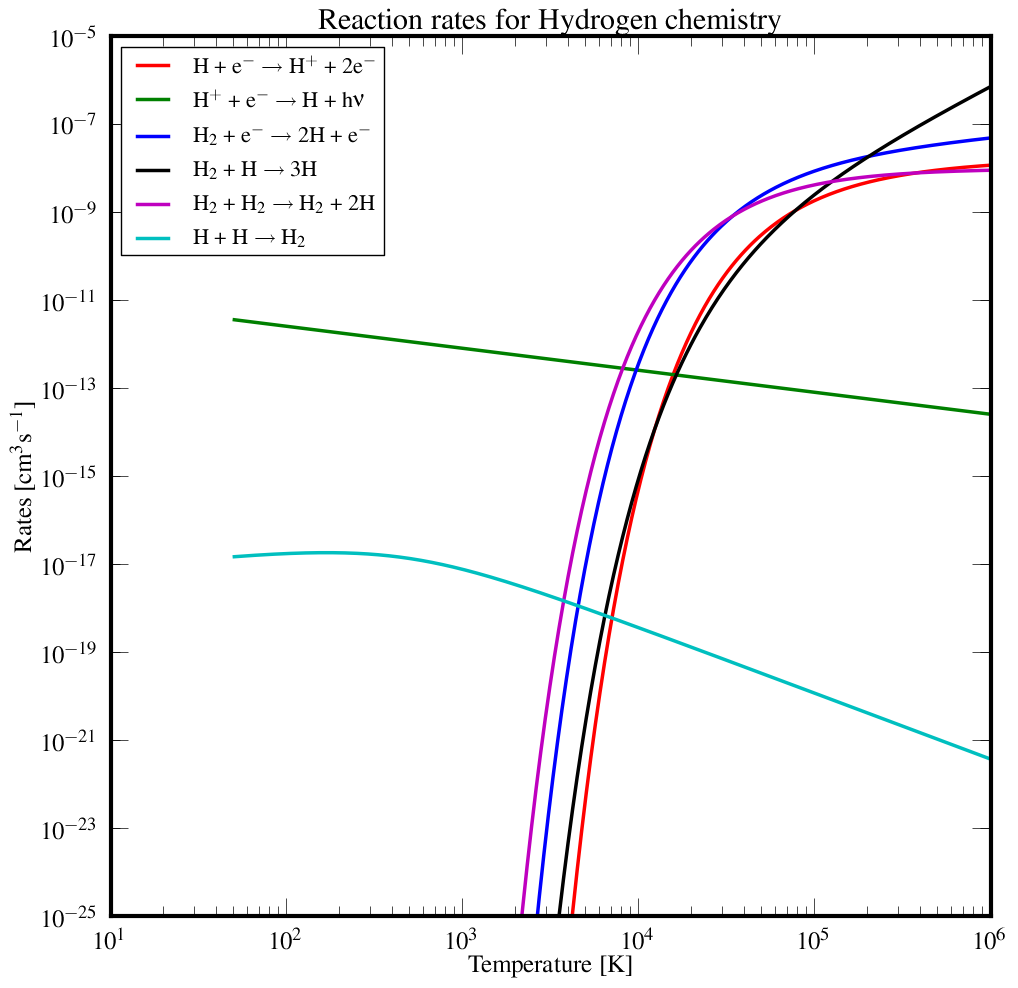
\includegraphics[width=1\columnwidth]{\figpath/H2ReactionRates.png}
 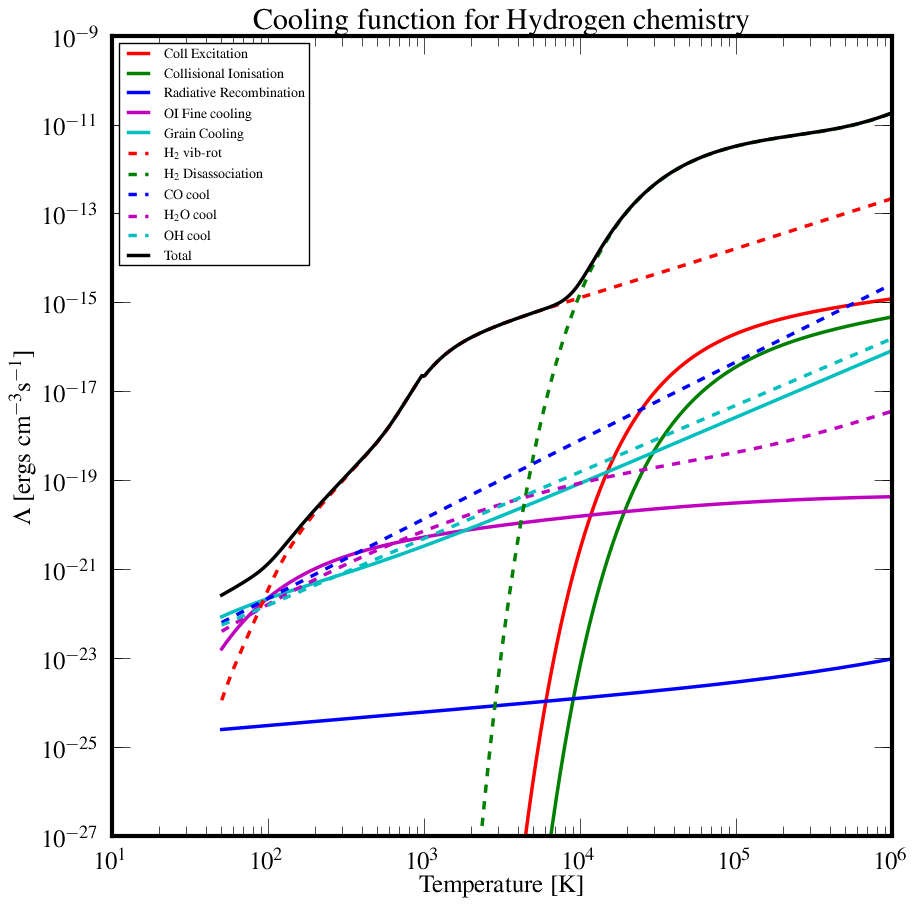
\includegraphics[width=1\columnwidth]{\figpath/H2CoolingFuncs.png}
 \caption{Variation of $H_2$ chemistry reaction rates, $k_{i}$ and cooling
   function $\Lambda(n,T,{\bf{X}})$ with temperature for the initial
   state (see Sect.~\ref{ssec:molcool})}
\label{fig:tempvar}
\end{figure*}

\begin{table*}
\begin{minipage}{\textwidth}
\caption{Summary of the chemistry reaction set. T is the temperature
  in Kelvin, $T_{\rm eV}$ is the temperature in electron-volts, $T_{5}$
  = $T/1\times10^{5}$  and 
$T_{2}$  = T/100}
\label{tab:chemeq}
\begin{tabular}{l l l l}
\hline
No. & Reaction & Rate Coefficient ($\rm {cm}^{3} s^{-1}$) &
Reference~\footnote{REFERENCES -- (1) \cite{Cen:1992p13616} [Eq. 26a];
  (2) \cite{Woodall:2007p13623} [UMIST Database] (3)
  \cite{Galli:1998p13066} [Eq. H17]; (4) \cite{Abel:1997p12836}
  [Tab. 3 Eq. 13]; (5) \cite{Hollenbach:1979p12707} [Eq. 3.8]}\\
\hline
1. & H + e$^{-}$ $\rightarrow$ H$^{+}$ + 2e$^{-}$ & $k_1$ = $5.85
\times 10^{-11}$ $T^{0.5}$ \rm{exp}(-157,809.1/T)/(1.0 + $T_{5}^{0.5}$) & 1\\
2. & H$^{+}$ + e$^{-}$ $\rightarrow$ H + h$\nu$ & $k_2$ =
$3.5\times10^{-12} (T/300.0)^{-0.8}$ & 2\\
3. & H$_{2}$ + e$^{-}$ $\rightarrow$ 2H + e$^{-}$ & $k_3$ =
$4.4\times10^{-10} T^{0.35} \rm{exp}(-102,000.0/T)$ & 3\\
4. & H$_{2}$ + H $\rightarrow$ 3H & $k_4$ = $1.067\times10^{-10}
T_{\rm eV}^{2.012}(\rm{exp}(4.463/T_{\rm eV})^{-1}((1. + 0.2472 T_{\rm eV})^{3.512})^{-1} $& 4\\
5. &H$_{2}$ + H$_{2}$ $\rightarrow$ H$_{2}$ + 2H & $k_5$ = $1.0\times 10^{-8} \rm{exp}(-84,100/T)$ & 2\\
6. & H + H $\overset{\rm dust}\longrightarrow$ H$_{2}$ & $k_6 =
3.0\times10^{-17}\sqrt{T_{2}}(1.0 + 0.4\sqrt{T_{2} + 0.15} + 0.2T_{2} + 0.8T_{2}^{2})$ & 5 \\
\hline
\end{tabular}
\end{minipage}
\end{table*}

\section{Radiative Transfer}
\label{sec:radtrans}
Radiative transfer modeling used for post processing.

\subsection{The radiative transfer code} \label{subsec:radiative_transfer_code}
The radiative transfer program used is LIME (LIne Modeling Engine; \citealt{Brinch:2010p13078}), which  calculates line intensities based on a weighted sample of randomly chosen points in a continuous 3D model. The method of selecting these points is given in section \ref{subsec:gridding}. At each of these points, the density of the main collision partner (equivalent amount of H$_2$, given by n(H$_2$)+ 0.5 n(H)), gas and dust temperatures, velocity, molecular abundances and unresolved turbulent velocity are specified. These points are then smoothed by Lloyd's algorithm \citep{Lloyd1982} in order to minimise the variation in distance between points whilst keeping the same underlying distribution. These points are then connected by Delaunay triangulation and it is between the points connected by this method that photon are allowed to propagate (fig.~\ref{grid}). The level populations of the selected molecules are calculated at each of these points from collisional and radiative (de)excitation and the local radiation field is calculated. This is repeated 20 times with the populations of each level converging towards a single value. This number of iterations is sufficient for the signal to noise ratio of the level populations (as defined in \citealt{Brinch:2010p13078}) to exceed 1000 for 99\% of the points, ensuring that the simulation has converged on a stable level population. After 20 iterations the model is ray-traced in order to produce synthetic brightness maps. The average of ten separate runs was taken to minimise the artefacts in the output images, resulting from the grid construction.% (Fig.~\ref{points}).


\begin{figure}
 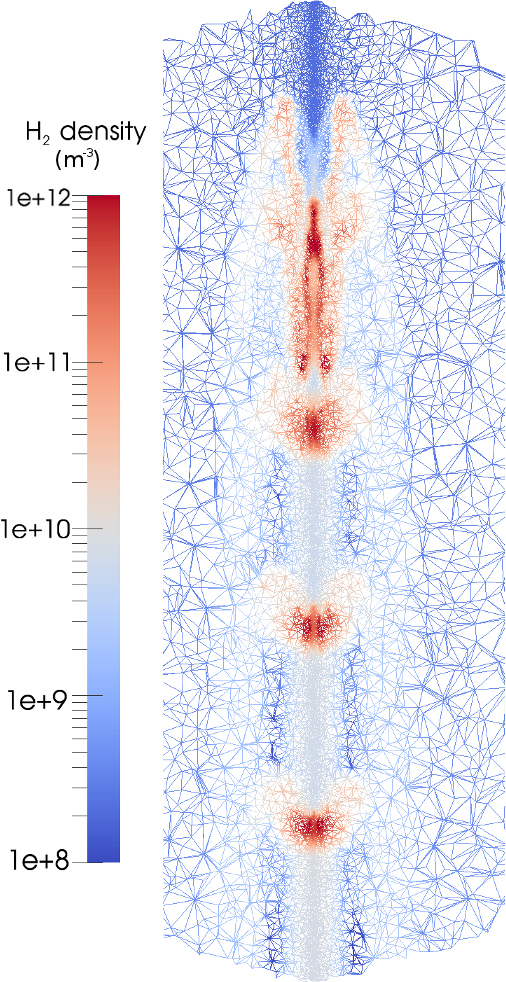
\includegraphics[width=84mm]{\figpath/grid.png}
 \caption{A plot of the points selected by the gridding process and the paths down which photons can propagate for points in the r,z plane. The points are color coded by the density distribution (in m$^{-3}$, as used in LIME) and are more concentrated in the high density knots.}
\label{grid} % This plots has to be changed. 
\end{figure}

\subsection{Grid construction} \label{subsec:gridding}
In order to construct the grid, candidate points are randomly selected from the volume to be simulated. These candidates then have their equivalent H$_2$ number density, and the number density of SiO, compared against those of a reference point in order to decide if the candidate point is to be used in the grid or not. Candidate grid points are selected at random in a cylindrical coordinates that is linearly spaced in z and $\theta$ and logarithmically spaced in r. For each point to be selected, a random number $\alpha$ is drawn from the semi-open set [0,$\,$1) as a threshold. After selection of random coordinates, the H$_2$ density and SiO density at the candidate point (n and m, respectively) are compared against the densities of a reference point in the un-perturbed ambient medium multiplied by $\frac{4\eta}{5}$ (n$_0$ and m$_0$). If $\alpha<\left( \frac{n}{n_0} \right)^{0.3}$ or $\alpha< \left( \frac{m}{m_0} \right)^{0.3}$ then the point is selected for use. Otherwise another r, $\theta$, z co-ordinate is selected and it becomes the candidate point. In addition to this method of selection, 5\% of the points are linearly distributed in x, y and z with no bias with regards to density or abundance. This provides a minimum level of sampling for the large low density regions in the outer parts of the simulated volume. %See fig. \ref{points} for an example of the points distribution in r, z. The function comparing the candidate point to the reference point and the candidate point distribution were selected empirically to sample all scales while ensuring that the majority of points are located in the inner disc where the density is higher.  \smallskip

\subsection{SiO abundance}
\label{ssec:sioabun}
Molecular abundance is one of the important ingredients that is
required by the radiative transfer code described above. 
Typically, extremely low abundance of SiO is
found (n(SiO)/n(H2) $< 3\times10^{-12}$) in dark, dense clouds such
as TMC1 \citep{Ziurys:1989p14699,MartinPintado:1992p14309}. Whereas, in
outflows like L1448, SiO abundance can increase up to 10$^{-6}$ specially in
molecular bullets moving with a projected velocity of 60
km\,s$^{-1}$ \citep{Dutrey:1997p11185}. Thus, there is
a significant increase of 6 orders of magnitude from quiescent clouds
to outflows crowded with shocks. Production of
gaseous SiO due to slow C-type shocks has been suggested to occur via release of
silicon from grain cores and from grain mantles. Various stationary
shock models indicate a sudden abundance increase in SiO 
near a shock speed of 20-30\,km\, s$^{-1}$. However, several young
outflows have velocities of the order of 100 km\,s$^{-1}$ as in the present
case. Shocks due to such outflows will dissociate H$_{2}$ and will
become J ({\em{jump}}) type shocks. Thus molecules observed in such
energetic outflows must have been reformed in the flow as suggested by
detailed models of J-shocks by \cite{Neufeld:1989p14322}. SiO formation in J shocks
have also been modelled recently and have thought to be reasonable
candidates of SiO line emission in molecular outflows and jets
\citep{Guillet:2009p11229}.
%

In-spite of all numerical models relating to the study of enhancement
of SiO in shocks, very little is known about the dependence of SiO
abundance on shock speeds. Considering the complex grain
chemistry that is involved in order to estimate the functional
dependence of SiO abundance on shock speeds, we prescribe these
profiles based on limited empirical evidences. The most simple among
them is the top hat profile in which the SiO abundance is a low value of
10$^{-12}$ below 20 km s$^{-1}$ and above 100 km s$^{-1}$ and a
maximum value of 10$^{-6}$ between these two velocities.
In order to get rid of a discontinuous change of abundance, we also
prescribe a gaussian such that the peak SiO abundance of 10$^{-6}$ is at
60\,km\,s$^{-1}$. While the value of n(SiO)/n(H$_{2}$) falls below
10$^{-9}$ at 20 and 100 km s$^{-1}$. These functional dependences of SiO
abundance on shock velocity are show in figure~\ref{abun}.  
In addition to this if the temperature at the point is greater than
92,000\,K (the temperature of the Si-O bond disassociation energy) 
the abundance is reduced to 10$^{-12}$. 
%

\begin{figure}
 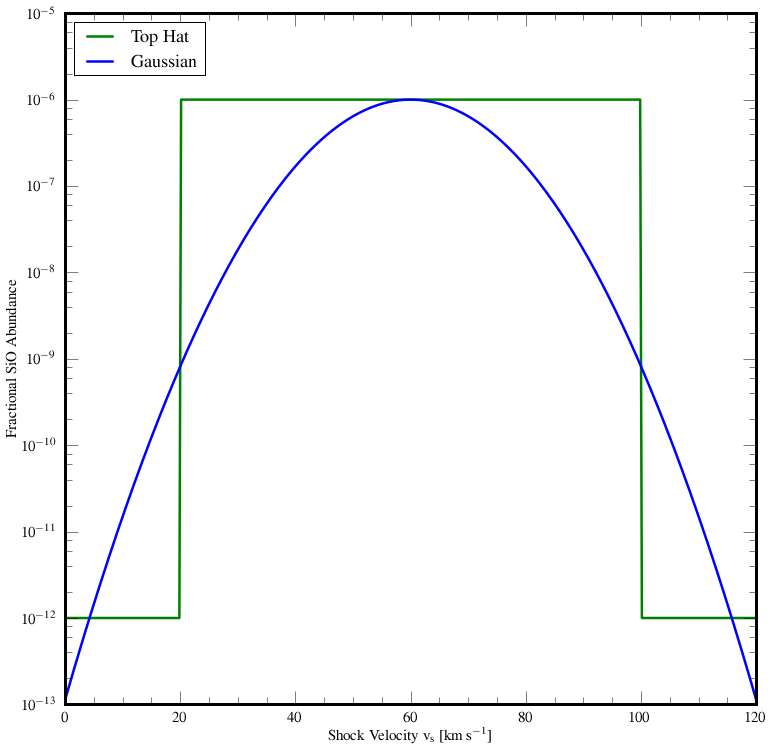
\includegraphics[width=1.\columnwidth]{\figpath/diffabunprof1.png}
 \caption{The different fractional SiO abundances as a function of
   shock velocity, v$_{\rm s}$.}
 \label{abun}
\end{figure}

Further, the velocities obtained from the dynamical simulations are in fact the
jet flow velocities. They can well be different from the shock
velocities depending upon the density contrast between the jet and
ambient medium. For the present study, we will consider two
cases. Firstly, the most simple one in which the jet flow velocity is
same as the shock velocity. Considering that there is a density
contrast in the simulation setup this assumption is will
overestimate the shock velocity. In order to correct the same we also
consider a case in which the shock speed of a dense plug accumulated
between the jet and medium is estimated by balancing the the respective ram
pressures \citep{Masson:1993p9661},
\begin{equation}
\label{eq:shockjetvel}
v_{\rm s} = \frac{v_{\rm j}}{1 + \eta^{-0.5}} = \frac{v_{\rm j}}{\delta}
\end{equation}
where v$_{\rm s}$ is the velocity of dense plug and v$_{\rm j}$ is the
jet velocity. A comparative view of using such velocity corrections and
functional forms of SiO abundances are discussed in
Sec~\ref{ssec:sioabunem}.

    

% The fractional abundance is given by the equation:

% \begin{eqnarray}
% log(X)=-2.48\times10^{-8}v^5 + 5.50\times10^{-6}v^4 \nonumber \\
% - 4.28\times10^{-4}v^3 + 1.24\times10^{-2}v^2 \nonumber \\
% + 2.52\times10^{-2}v - 1.20\times10^{1}
% \label{eq:fracSio}
% \end{eqnarray}

% where v is the shock velocity in kilometres per second. 




\section{Parameter Survey}
The results and analysis for the present work are divided in two parts,
viz., the dynamical numerical simulations and the post-processing with
radiative transfer code. For each part we have used certain parameters
and the effect of changing them is studied. Ideally all these parameters should come from observational
results. However, not all quantities needed for our study are well
constraint by the observations, thus allowing us vary them as
free parameters. Such a parameter survey provides better handle on the range of allowed
values on qualitative comparison with observations. 
%

\subsection{Parameter definitions}
\label{ssec:paradef}
For the first part of the study concerning the dynamical numerical
simulations, we will focus on two main parameters. They are the
prescription of cooling and the density contrast between the jet and
the ambient medium denoted by $\eta$. The various cooling prescriptions used for the present study are
described in details in section~\ref{sec:chem}. They differ in the
physical process that is responsible for cooling and chemistry. The
most simple one is that of power-law cooling with no chemistry and the
most complex cooling module is where molecular hydrogen chemistry is
evolved with contributions to cooling from other abundant molecules
like CO, OH etc. 
%

A value of $\eta > 1$, mean that
that jet is over dense with respect to the medium. In all our runs with
different cooling prescriptions, we have assumed the jet to be
over-dense by 10 times that of the ambient medium. Additionally, for
the atomic, tabulated and molecular cooling runs we have used a
value of $\eta$ of the order of unity indicating similar densities in
the jet and the medium. 
The magnetic field strength is kept to be fixed using $\beta = 10.0$,
for all our runs. Table~\ref{tab:result1} lists all the runs with
varying $\eta$ and cooling prescriptions, along with the peak
intensity and line widths at the bow shock.
%

To obtain the SiO emission maps and corresponding
spectra, two additional free parameters are required along with other
inputs described in section~\ref{sec:radtrans} . They are
the fractional abundance profile of SiO and the angle of inclination with
respect to line of sight denoted by $\phi$. Section~\ref{ssec:sioabun}
describes all the profiles used for the present study. The obvious
choice for the inclination angle, $\phi$ is 90$^{\circ}$ indicating
the outflow is in the plane of the sky. 
Additionally, we have used two other angles of inclination apart from the
plane of the sky, i.e, $\phi = 45^{\circ}, 60^{\circ}$ to compare
results with observations. The runs with different fractional
abundance profiles are described in table~\ref{tab:result2}. A
parameter introduced here is $\delta$ which is essentially the ratio
of shock velocity v$_{\rm s}$ and initial jet velocity v$_{\rm
  j}$ such that its value depends on density contrast $\eta$
(see Eq.~\ref{eq:shockjetvel}).

\begin{table*}
\centering
\caption{Summary from parameter runs.}
\begin{tabular}{c | c | c | c | c | c | c }
\hline
Run & Cooling Mode & $\eta$ & \multicolumn{2}{|c|}{Top Hat Profile
  $\delta = 1$} & \multicolumn{2}{|c|}{Gaussian Profile $\delta =
  1$}\\
\hline\hline
&&& $\int T_{\rm MB}dV$ [K-km\,s$^{-1}$] & $\Delta$v [km s$^{-1}$] & $\int T_{\rm MB}dV$ [K-km\,s$^{-1}$] & $\Delta$v [km s$^{-1}$] \\
\hline
adi1010 & Nil (Adiabatic) & 10 & 2.91 & $>$40 & 0.25 & 40.0 \\
pow1010 & Power law & 10 & 0.64 & 8.0 & 0.02 & 10.0\\
atm1010 & Atomic & 10 & 2.04 & 36.0 & 0.58 & 38.0 \\
atm210 & Atomic & 2 & 3.21 & 18.0 & 0.64 & 20.0 \\
tab1010 & Tabulated & 10 & 0.75 & 11.0 & 0.09 & 10.0 \\
tab210 & Tabulated & 2 & 2.89 & 8.0 & 1.0 & 9.0 \\
mol1010 & Molecular & 10 & 1.10 & 10.0 & 0.1 & 11.0 \\
mol310 & Molecular & 3 & 3.3 & 14.0 & 0.66 & 12.0\\
\hline
\end{tabular}
\label{tab:result1}
\end{table*}


 

\begin{table*}
\centering
\caption{Summary of radiative transfer runs with different SiO fractional abundance
  profiles for dynamical simulation with molecular cooling and
  $\eta=3$. The integrated intensity of the brightest lobe assuming a single disk
  observation with a beam width of $15\,\arcsec$ is listed along with the
  corresponding spectral width.}
\begin{tabular}{l | l | l | l | l}
\hline
Profile & $\delta$ = v$_{\rm jet}$/v$_{\rm s}$ & $\int T_{\rm MB}dV$
[K-km\,s$^{-1}$] & $\Delta$v [km s$^{-1}$]\\ 
\hline\hline
Top Hat & 1.0 & 3.3 & 14.0 \\
Top Hat & 1/$(1.0 + \eta(z)^{-0.5})$ & 4.9 & 14.0 \\
Gaussian & 1.0 & 0.66
& 12.0 \\
Gaussian & 1/$(1.0 + \eta(z)^{-0.5})$ & 1.1
& 12.0 \\
%Functional & 100.0 & $(1.0 + \eta(z)^{-0.5})$ &
%& \\
%Functional & 100.0 & $(1.0 + \eta(z)^{-0.5})$ &
%& \\
\hline
\end{tabular}
\label{tab:result2}
\end{table*}

\subsection{Reference Run}
\label{ssec:refrun}
We define a reference run in order to quantify and compare results obtained from such a
survey of above mentioned parameters. The results shown in this work will be
pertaining to the reference run and appropriate comparison will be
discussed with other runs.
%

The reference run in our calculation has density contrast $\eta$ = 3
with a plasma beta, $\beta$ = 10. The jet for this run is 89\% atomic,
10\% molecular and 1\% ionized to begin with. This jet enters the
ambient medium with a velocity of v$_{\rm jet,0}$ = 100 km
s$^{-1}$. The cooling in the jet is
via molecular cooling prescription, whereby the hydrogen fractions are
evolved with cooling contributions for abundant molecules like CO, OH
etc. The steady state density, temperature and velocity obtained from this 
run is post-processed to obtain the observational features
corresponding to SiO molecule. 
For the radiative transfer calculation, the source in the reference
run is stationary and the jet is in plane of the sky ($\phi =
90^{\circ}$). A gaussian profile is used for the fractional abundance
of SiO.
%TheSiO fractional abundance used is that obtained
%from equation~\ref{eq:fracSio}. 
Further, the shock velocity which determines
the fractional abundance, v$_{\rm s}$, is less than the jet velocity in the
flow, such that their ratio $\delta$ is given by 1./$(1.0 +
\eta(z)^{-0.5})$, where $\eta(z)$ is the density contrast as a
function of height from the base of the jet.

\section{Results}


\subsection{Comparison of cooling prescription}
\label{ssec:coolres}
Importance of cooling prescriptions\\
Bulk of emission comes from cooling instabilities.
figure nos. 2 -- Simulated images, emission maps for eta = 10.
\begin{figure*}
 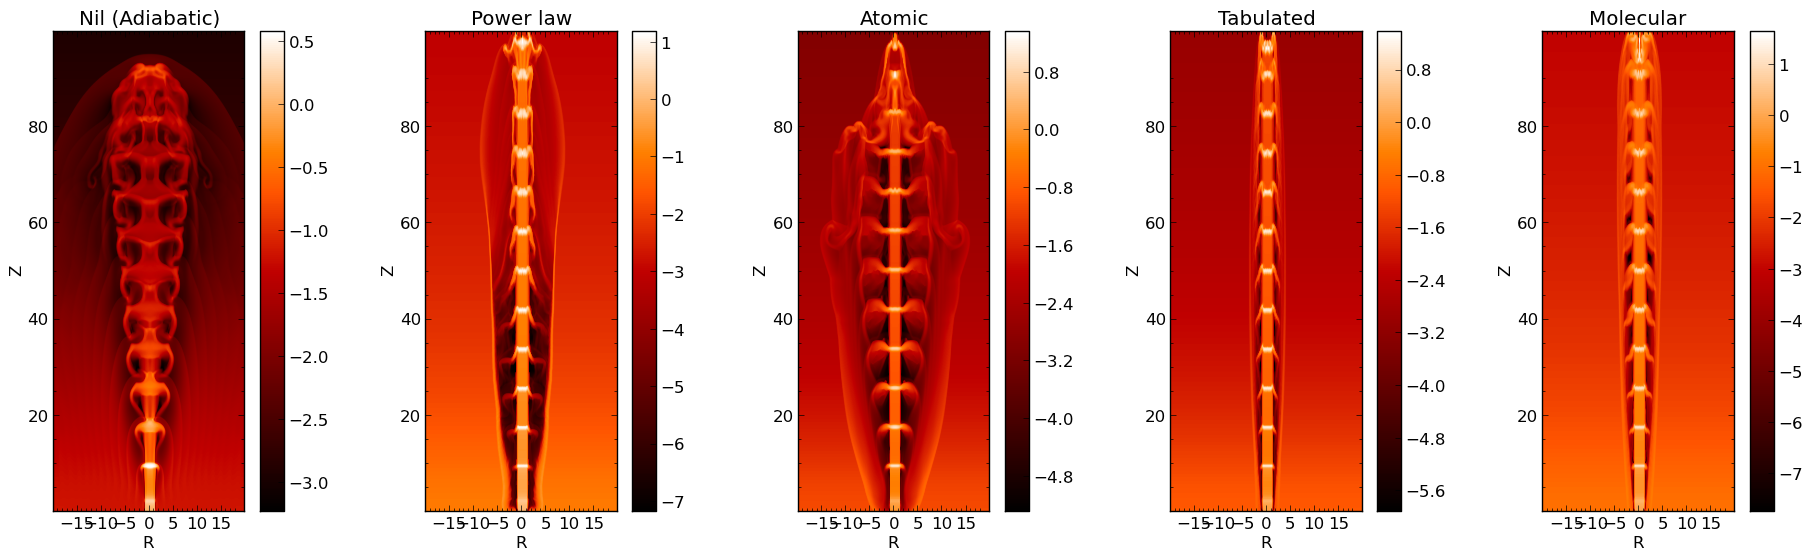
\includegraphics[width=2.\columnwidth]{\figpath/jetplt1_1010.png}
 \caption{Jet Volume Density for different cooling modes with
   $\eta$ = 10 and $\beta$ = 10.}
\label{grid}
\end{figure*}

\begin{figure*}
 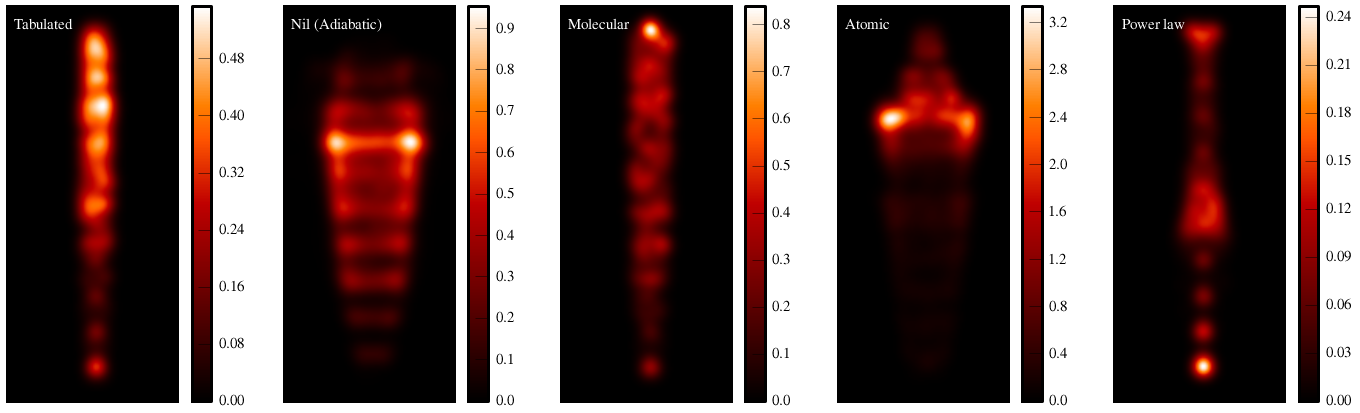
\includegraphics[width=2.\columnwidth]{\figpath/diffcool_EMgaussprof.png}
 \caption{A plot of the integrated SiO J2-1 emission from 5 models, 
each using a different method to calculate cooling and all with $\eta$=10 $\beta$=10.}
\label{cooling2-1} 
\end{figure*}


% \subsection{Effects of changing $\eta$ and $\beta$}
% figure nos. 2 -- Simulated images describing lengths, collimation and
% emission for lower eta more stronger. 
% \begin{figure*}
%  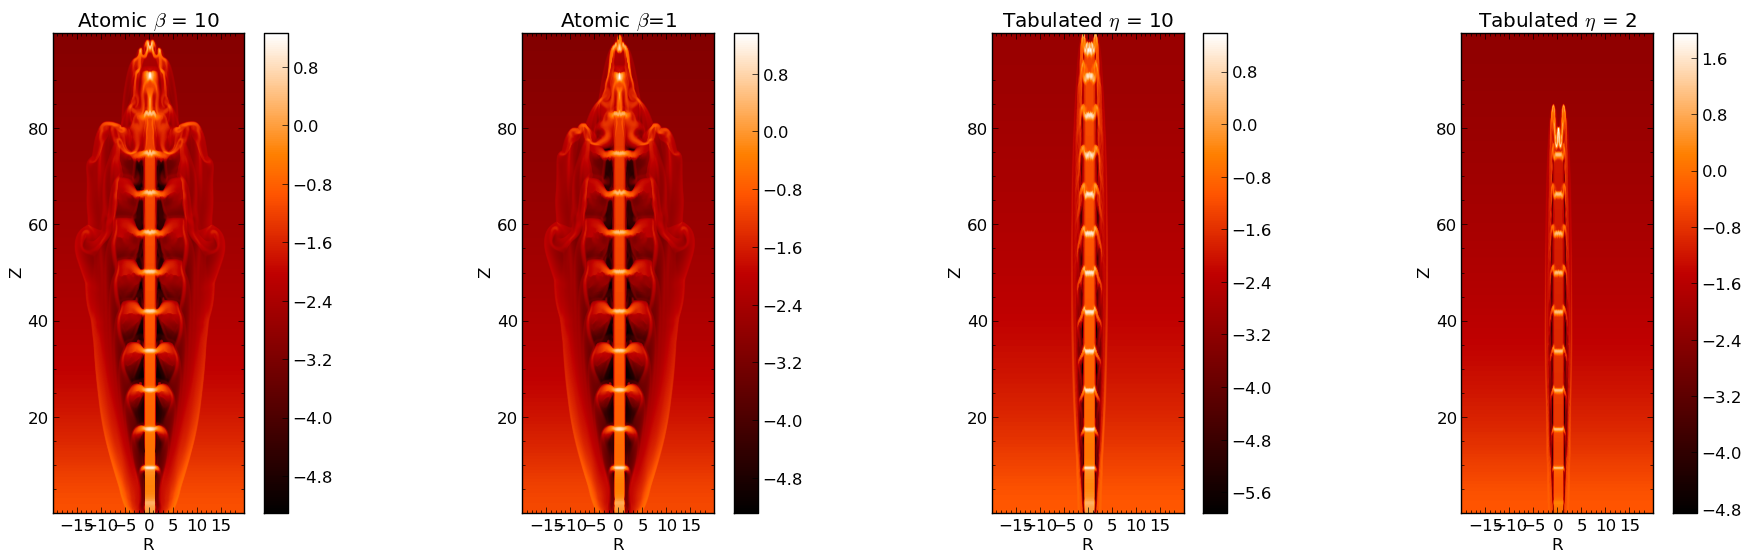
\includegraphics[width=2.\columnwidth]{\figpath/jetplt2_diffetabeta.png}
%  \caption{Jet Volume Density for atomic cooling with $\eta$ = 10 but $\beta$ = 1 and
%    10 and that with tabulated cooling with $\beta$ = 10 but $\eta$ = 2
%    and 10.}
% \label{grid}
% \end{figure*}

\subsection{Molecular cooling and H$_2$ Chemistry}
In case of molecular outflows, the most appropriate form of cooling
prescription among the ones described in sect.~\ref{sec:chem} is
that which involves the evolution of H$_2$ chemistry along with
contributions to cooling from fixed fractions of other molecules like
CO, OH etc. First three panels of figure~\ref{fig:Hfracsim} shows the density of
various hydrogen species in the outflow for the simulation run with
$\eta$ = 3 and $\beta$ = 10. The jet is largely dominated by atomic
and molecular hydrogen, however, the fraction of these species have
considerably changed from their initial values within the
jet. Ionized hydrogen is mainly formed at the tip
of the bow as seen by the increase of fHII to 10\% from an initial value of
1\% within the jet.
%
 
The last two panels of figure~\ref{fig:Hfracsim}
show the temperature and mean molecular weight $\mu$. The
highest temperature of $\sim$ 50000\,K is attained in our flow at the
tip of the bow shock. While the temperature on the edges (i.e.,interface between
jet and the ambient medium) is lower than 5000\,K. Also the relatively
weaker shocks formed due to knots do not heat up the material beyond
few 10$^{3}$\, K. The mean molecular weight, $\mu$, gives an indication
on which specie of hydrogen dominates in what regions of the flow. In
particular, a value of $\mu > 2.$ represents regions dominated by
molecular hydrogen, while regions close to the bow shock have lowest
values of $\mu$ where ionized hydrogen is present and along the jet the value
$\mu$ is close to 1.3 suggesting an atomic jet. 
%

\begin{figure*}
 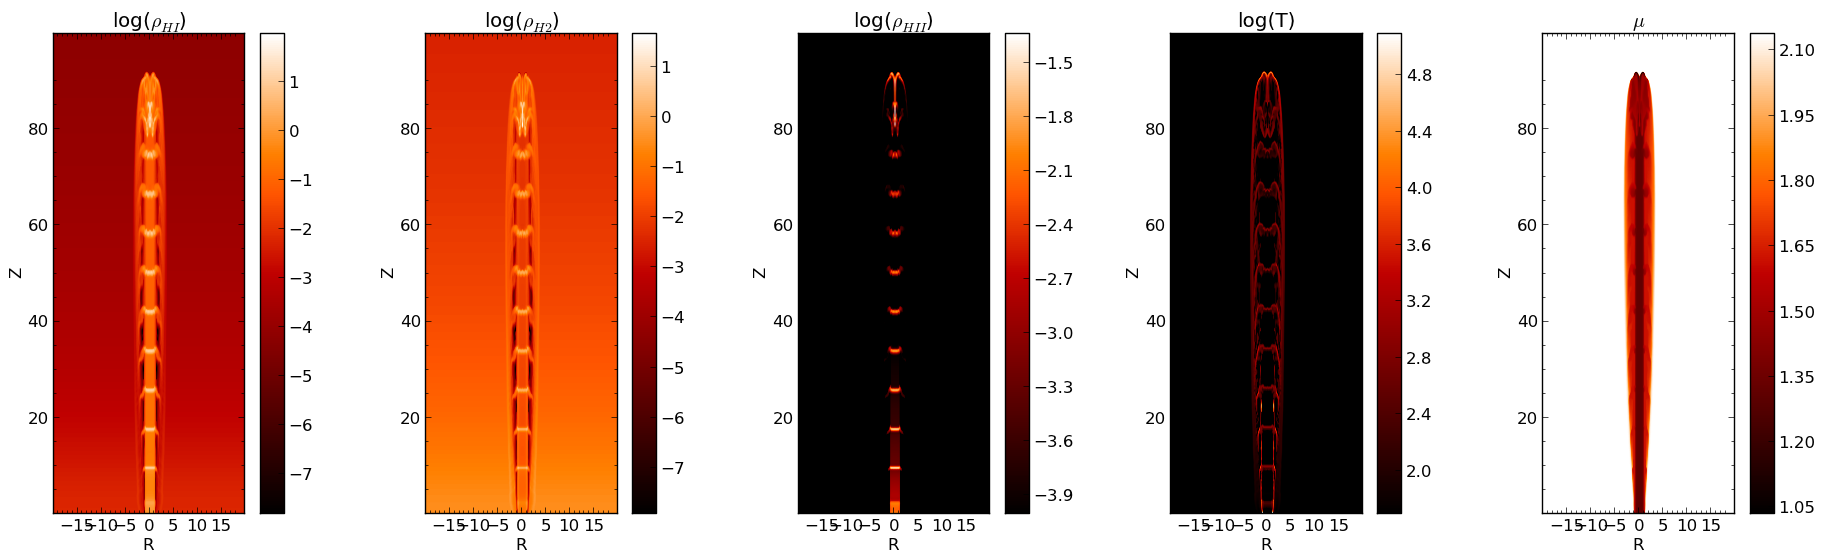
\includegraphics[width=2.\columnwidth]{\figpath/molcjet_310.png}
 \caption{Fraction of hydrogen species in the run with molecular
   cooling having $\eta$ = 3 and $\beta$ = 10.}
\label{fig:Hfracsim}
\end{figure*}


The distribution of fractions of different hydrogen species along with
temperature suggests that there are essentially three regions where
chemistry is evolved due to shocks.
They are : (1) The tip of the jet , (2) The edges of the jet and
(3) intermediate knots. As the atomic jet propagates from the lower boundary 
into the cold molecular medium , it forms a strong shock resulting in
forming a density and temperature discontinuity. Such a jump in
dynamical quantities play a crucial role in evolution of
chemistry. For example, temperatures beyond few 1000\,K produced in the shocks could
disassociate the molecules and can also lead to ionization if
temperature reaches above 10$^{4}$\,K.
%
\begin{figure*}
 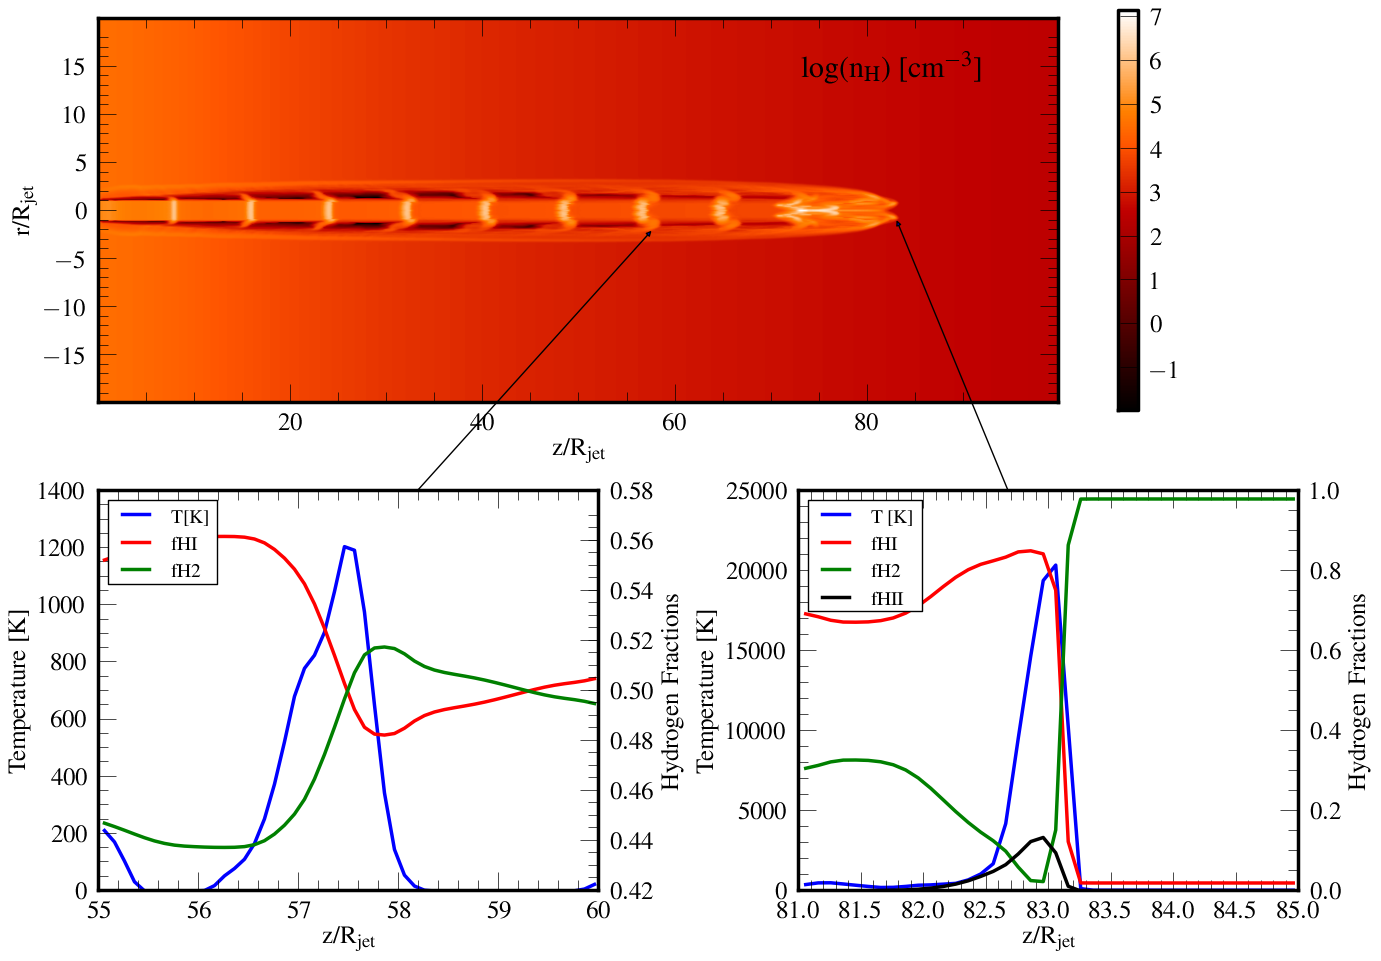
\includegraphics[width=2.\columnwidth]{\figpath/molcjet_310_molform.png}
 \caption{Dependence of hydrogen fractions on the temperature at two
   points in the flow, viz. the interface of the knot with molecular
   medium and at the bow shock}
\label{fig:Hmolform}
\end{figure*}

For the reference run, the effect of shock in dynamical evolution of
hydrogen fraction is presented in figure~\ref{fig:Hmolform}. The top
panel of the figure shows number density of hydrogen in the jet. This
hydrogen exists in three forms namely, molecular, atomic and
ionized. The fraction of each of these forms are shown in bottom
panels of figure~\ref{fig:Hmolform} at two representative regions in
the jet marked with the arrow. The left bottom panel shows the
vertical distribution of temperature, molecular and atomic fraction at the
interface of the knot and the ambient medium. The interaction of the
knot with the medium raises that temperature to 1200\,K and
accumulates the matter such the density in that region reaches up to
10$^{6}$ cm$^{-3}$. Behind the shock as the material cools, atoms
combine together to form molecules as seen in the increase of fH2 from
0.44 to 0.52. This rise in molecular fraction comes at an expense of
reduction in atomic fraction from 0.56 to 0.48. Further away from the
shock, these species tend to reach a quasi equilibrium as their
fractions reach towards a value of 0.5. The ionized fraction is
extremely low in this region due to low temperatures. However at the
bow-shock, temperatures rise up to 20000\,K. Molecular
hydrogen species are destroyed, while ionized hydrogen shows an
increase in its fraction as seen in the bottom right panel of
figure~\ref{fig:Hmolform}. The peak in ionized fraction of 0.15
coincides with the peak in temperature profile as expected. The
molecular fraction shows a considerable dip from 0.3 to 0.03 at 
this temperature before rising sharply in the ambient molecular
medium. 
%

In summary, the axi-symmetric jet flow with periodic knots 
produce shocks of varied strengths giving rise to density, velocity and
temperature distribution. Molecular cooling and chemistry also 
allows us to evolve fractions of different hydrogen species along with the jet
flow. These jet quantities are then post-processed with a radiative
transfer code described in section~\ref{sec:radtrans} to obtain emission maps,
spectra and PV diagrams.



\subsection{Emission Maps, Spectra and PV diagrams}
\label{ssec:emspecpv}
The output obtained from the radiative transfer calculation is a data
cube with velocity being the third axis. This allows us to obtain
spectra and position velocity diagrams from these data cubes. 
Figure~\ref{empvspec90} shows all the possible outputs from the data
cube for the J = 2-$>$1 transition for the reference run. 
The top left panel in the figure shows the emission map for the jet
directed downwards. The notable features are the knots close to the
base of the jet and the emission near the bow shock due to density
enhancement by cooling instability. The PV diagram shown in the top
right panel is obtained along the jet as indicated by vertical magenta
line. The position is shown in terms of pixels, where each pixel has a
width of about 16\,AU. The channel numbers in the X-axis indicate
velocities. The whole velocity range of -20 km s$^{-1}$ to 20 km
s$^{-1}$ is uniformly divided into 80 channels. High velocity features
are clearly seen in regions corresponding to the knots in the emission
maps. These features fade along the jet as the knots also disappear in
the emission map. The region close to the bow shock as well gives
indication of high velocity features which are seen as broad wings in
the spectra. 
%

\begin{figure}
 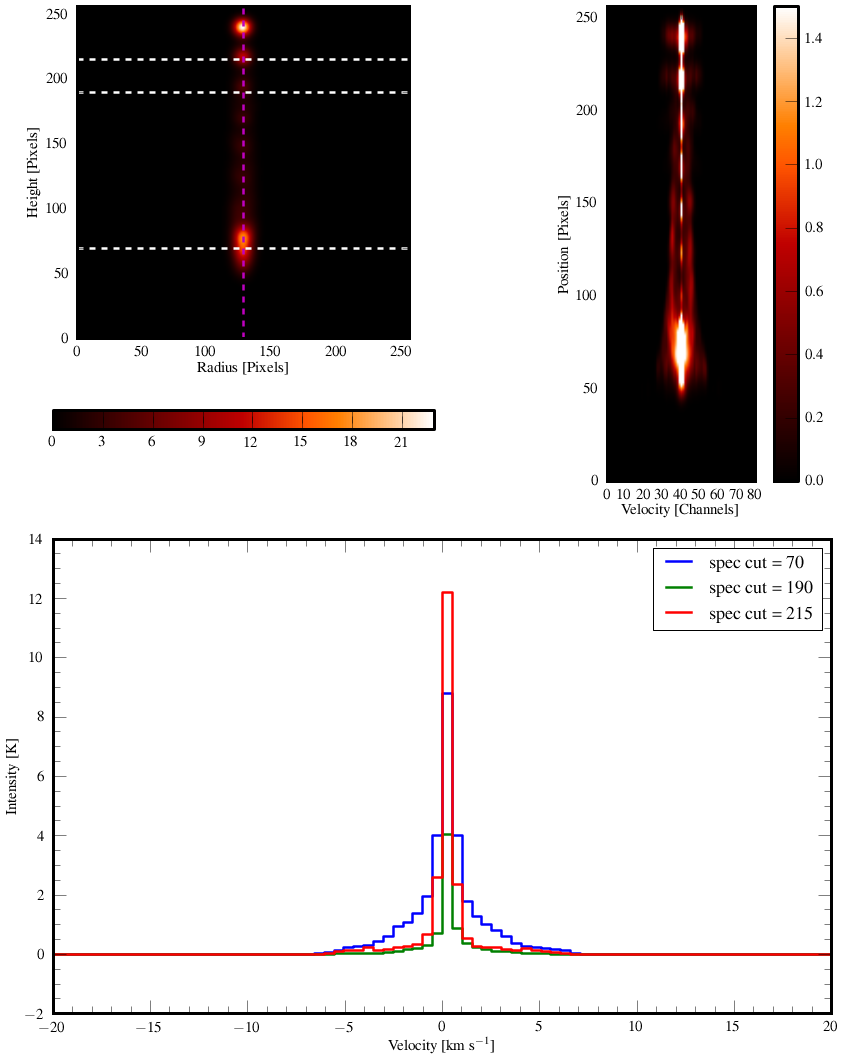
\includegraphics[width=1.\columnwidth]{\figpath/refrun_21_90_emspecpv.png}
 \caption{Integrated Emission map ({\it top left}), PV diagram ({\it top right}
   and spectra ({\it bottom} for the
   2-$>$1 SiO transition for the reference run. 
   The jet is assumed to be in the plane of sky implying an angle of
   inclination of $90^{\circ}$. The horizontal
 {\it white dashed} line marks the cuts where the spectra is taken
 while the vertical {\it magenta dashed} line represents the cut for
 the PV digram.} 
\label{empvspec90}
\end{figure}

The spectra at three different positions in the flow are shown in the
bottom panel of figure~\ref{empvspec90}. These three positions are
basically the two knots close to the base of the flow and region close
to the bow shocks. They are marked by horizontal white dashed lines in
the emission maps. The knot closer to the base is the brightest
showing a peak intensity of 50\,K. As one moves along the jet the
intensity decreases and reaches to about 10\,K close to the bow shock.
The line widths seen for this reference run with an angle of
inclination of 90$^{\circ}$ are typically around 5-10 km s$^{-1}$.
These line widths increase substantially as the angle of inclination
decreases. Figures~\ref{empvspec60} and \ref{empvspec45} show the
emission map, PV diagram and spectra for the same reference run but
with angle of inclination of 60$^{\circ}$ and 45$^{\circ}$
respectively. These runs are done assuming the the source has a
velocity of 20 and 30 km s$^{-1}$ respectively.
The spectra for low inclination angles are much broader
and less bright at the same three positions in the flow (shown by
three white dashed lines). The line 
widths now are typically of the order of 20 km s$^{-1}$ and the peak
intensity of the brightest knot is approximately 10\,K. 
The PV diagrams in these runs are not anymore symmetric unlike the run
with the jet in plane of the sky. Instead, they show a distinct {\it zig-zag}
pattern at each of the knots and region close to the bow shock.


\begin{figure}
 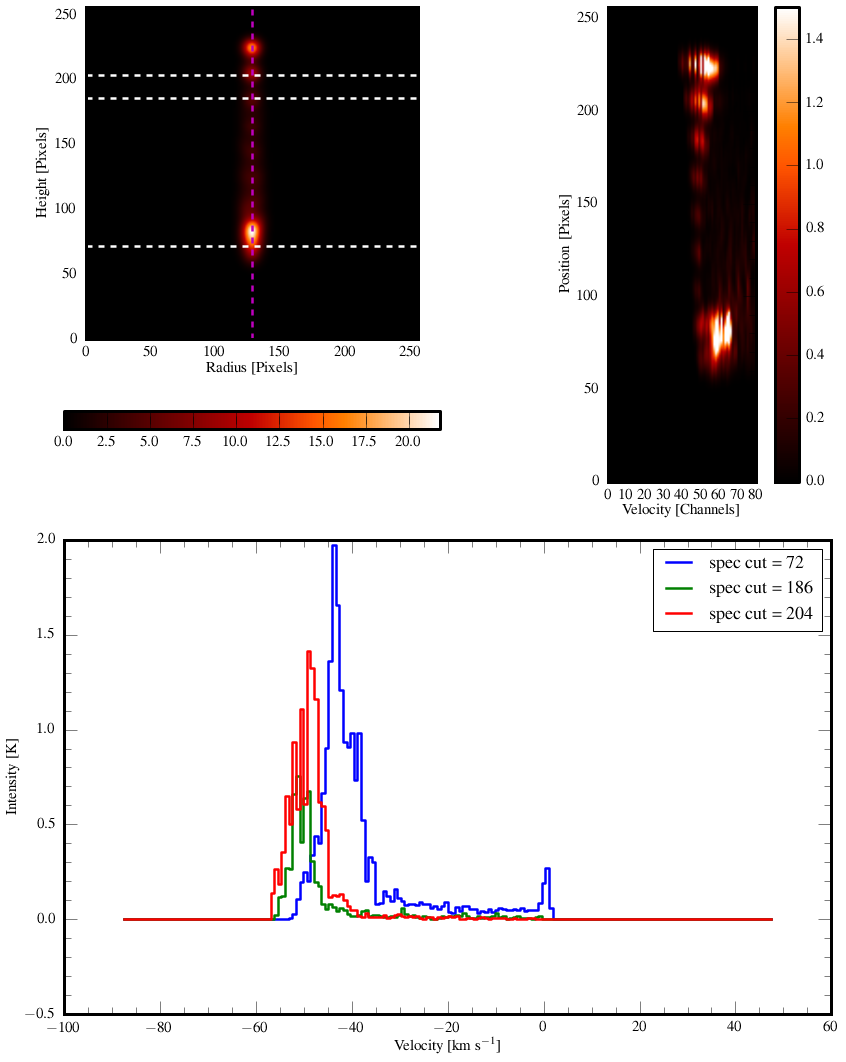
\includegraphics[width=1.\columnwidth]{\figpath/refrun_21_60_emspecpv.png}
 \caption{Same as figure~\ref{empvspec90} but with angle of
   inclination of $60^{\circ}$.} 
\label{empvspec60}
\end{figure}

\begin{figure}
 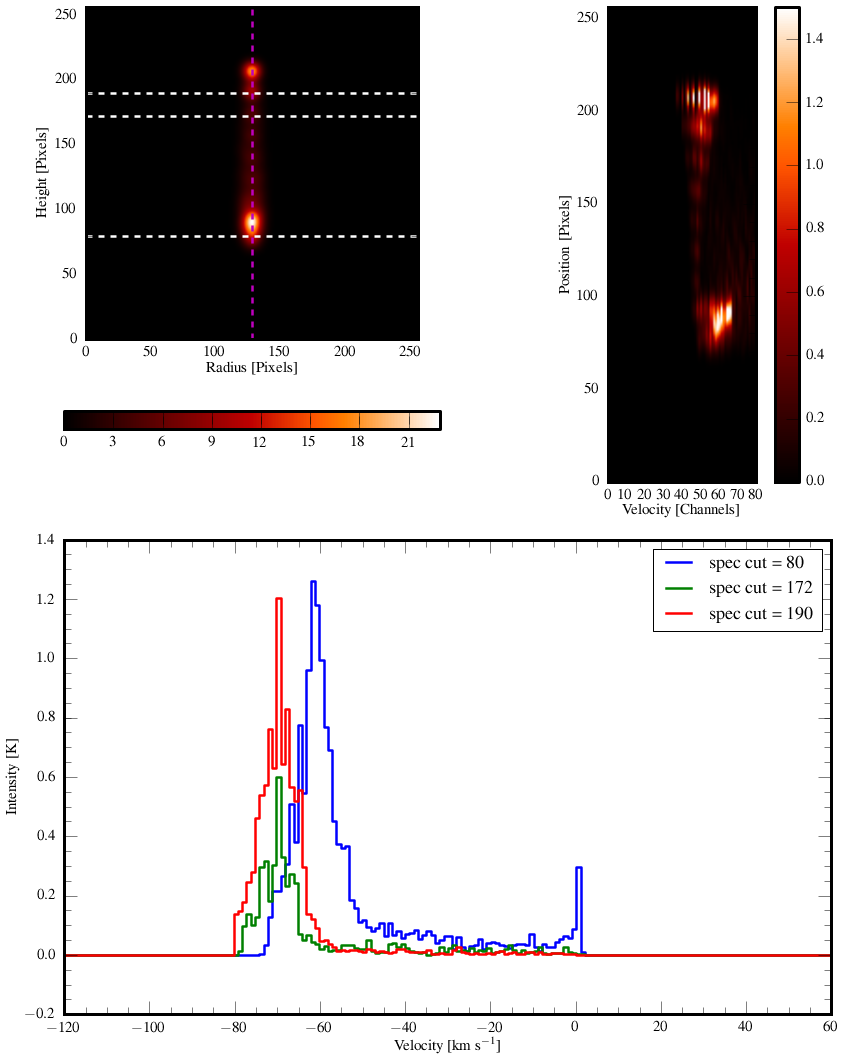
\includegraphics[width=1.\columnwidth]{\figpath/refrun_21_45_emspecpv.png}
 \caption{Same as figure~\ref{empvspec90} but with angle of
   inclination of $45^{\circ}$.} 
\label{empvspec45}
\end{figure}

%
The predicted emission maps, spectra and PV diagrams are shown above to depend
on the angle of inclination. In the next section, we focus on the
dependence of these observational features on the 
different fractional abundance profiles of SiO.



\subsection{SiO Abundance profile}
\label{ssec:sioabunem}
Input profiles in the radiative transfer code for the
fractional abundance of SiO are a very modest approximation from 
observed values (see sec~\ref{ssec:sioabun}). In
figure~\ref{fig:diffabunem}, we compare the maps for J = 2-$>$1
emission for two different abundance profiles and ratio of jet to
shock velocities. There is a striking difference with regards to
emission from the internal knots in these images. All the internal
knots show emission in the J=2-$>$1 line whilst using a top hat profile
and accounting for shock speeds (i.e. $\delta < 1$). However, some of
these knots are not observed when using the same top-hat profile but
assuming the shock velocity to be same as the jet velocity (i.e.,
$\delta$ = 1). Similar qualitative characteristics are seen in case of a gaussian
abundance profile. In particular, the case with $\delta$ = 1 only
produce emission from the knot closest to the bow shock, while the internal
knots do not show any appreciable emission. Further, the emission from
the knot closer to the bow shock varies considerably with different
profiles and value of $\delta$. It is the brightest for the case with
a top-hat profile and $\delta < 1$. The peak emission and line widths at this knot
are listed in table~\ref{tab:result2}
%

\begin{figure*}
 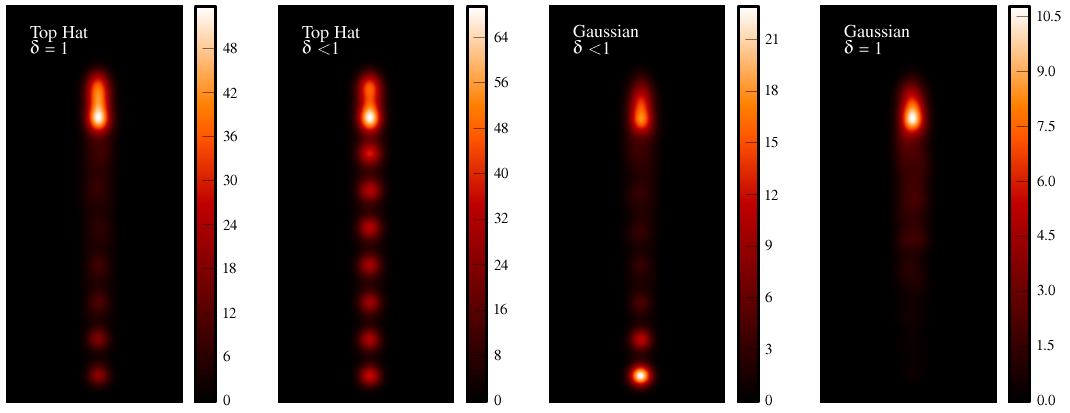
\includegraphics[width=2.\columnwidth]{\figpath/EM_gaussandth.png}
 \caption{Variation of 2-$>$1 SiO emission for runs with molecular
   cooling having $\eta$ = 3 and $\beta$ = 10 and different abundance profiles.}
\label{fig:diffabunem}
\end{figure*}


The dependence of emission on SiO abundance profile is expected due to
the distribution of jet velocity obtained from dynamical
simulations. We see that the velocity of internal knots lie around
70-90\,km\,s$^{-1}$, while the pulsed jet was injected with a mean of
100\,km\,s$^{-1}$. The knots slow down during the evolutionary
phase as they interact with the ambient medium. Interestingly, younger
knots closer to the base of the jet are brighter compared to older
ones further away from the jet (see panels 1 and 3 of
fig~\ref{fig:diffabunem}). This is attributed to the fact that the
ambient medium has a density gradient that goes as $\sim
z^{-2}$. Thus, the younger knots suffer the most deceleration closer
to the base of flow. This fact is taken into account when the shock
velocity is consistently calculated using the density contrast and
using a value of $\delta <$ 1. This process is further validated by
the lack of emission from internal knots in panel 4 of the
fig~\ref{fig:diffabunem}. 
%

Additionally, the internal knots show their distinct signatures in
form of {\em Hubble wedges} as seen in the PV diagrams for these
different profiles (see
~\ref{ssec:emspecpv}). Figure~\ref{fig:pvdiffabun} shows a zoomed
version of the bottom four internal knots in form PV diagram for these
different abundance profile. As expected, the signatures of knotty
emission is missing for the case with gaussian profile with $\delta$ =
1. Further, the wedges formed in panels 1 and 2 of the figure in
general slightly more extended in position space as compared to ones
formed in panel 4 of the same figure. This is indeed because of the
discontinuous nature of top-hat abundance profile as the SiO is
enhanced to a maximum abundance for all velocities between 20 and 100
km\,s$^{-1}$, which is not the case in a more continuos gaussian
distribution.

\begin{figure*}
 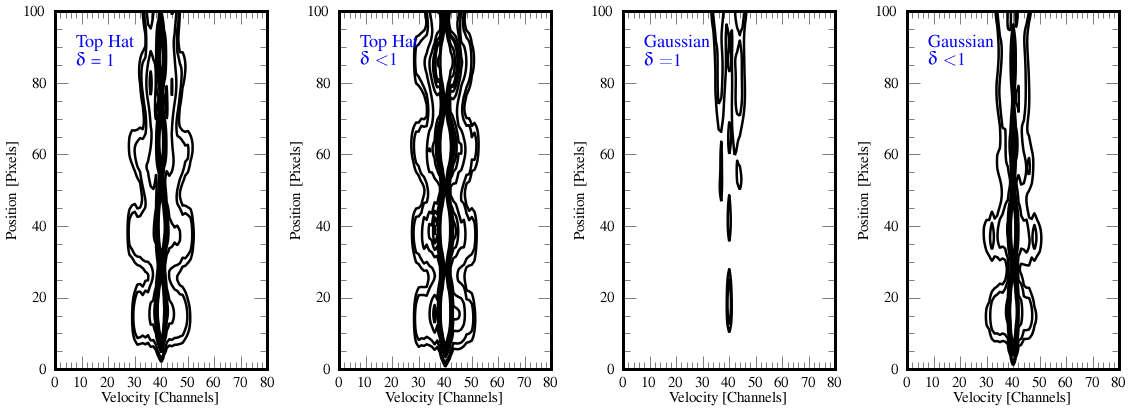
\includegraphics[width=2.\columnwidth]{\figpath/PV_gaussandth.png}
 \caption{Contour maps of position-velocity diagram for the internal
   knots for 2-$>$1 SiO emission for runs with molecular
   cooling having $\eta$ = 3 and $\beta$ = 10 and different abundance
   profiles. The contours mark different levels of emission in Kelvins, viz.,
   0.2,0.6,1.0,1.4,1.8,2.0,3.0,4.0.}
\label{fig:pvdiffabun}
\end{figure*}
   
 
\section{ALMA view}
ALMA view of the reference run and stress of applying our synthetic techniques
to study the molecular outflows in more details.\\

In order to see the interior structure of the molecular outflow, high resolution interferometric observations are needed. To demonstrate how jets similar to those we have modeled would look through such observations we have performed synthetic Atacama Large Millimetre Array (ALMA) observations using the Common Astronomy Software Applications package (CASA). The output from the radiative transfer were scalled to 300pc and used as the sky models for observations of the J=2-1, J=5-4 and J=8-7 lines at freqencies of 86.85, 217.10 and 347.33$\,$GHz, which fall in ALMA bands 3, 6 and 7. The observations were simulated using cycle 1 ALMA for 30 minutes total integration time, in the configurations c32-6, c32-4 and c32-3 for the three lines, giving beam sizes of 0.72'', 0.47'' and 0.58'' and sensitivities of 0.05, 0.07 and 0.09$\,$mJy/beam for the three lines (as calculated by the ALMA online sensitivity calculator) with velocity resolutions of $sim$1$\,$km/s.

\begin{figure*}
 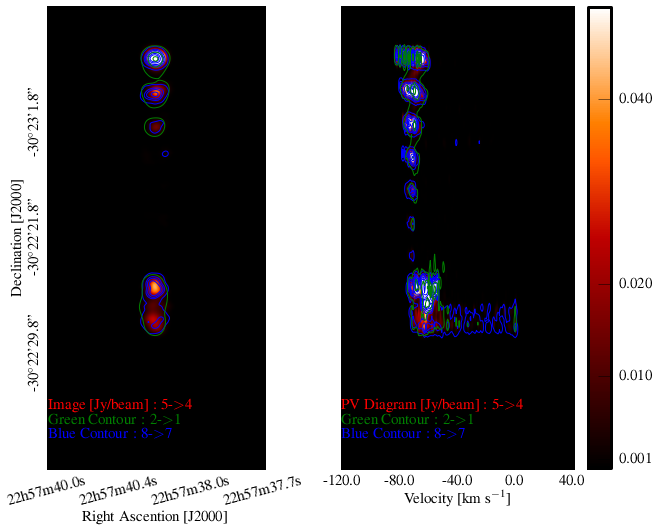
\includegraphics[width=2.\columnwidth]{\figpath/ALMAmaps2.png}
 \caption{{\bf Left:} The intensity map in the channel of the peak of the J5-4 emission. The heat map shows the 5-4 line intensity, the blue contours show the J=8-7 line intensity and the green contours show the J=2-1 line intensity (both in steps of 10mJy/beam) (this is arbitrary, could we do integrated intensity here instead?). {\bf Right:} The PV diagram taken along the axis of the jet, showing a 'zig-zag' pattern between the knots of the jet and broad emission at the bow shock.}
\label{fig:almafig}
\end{figure*} 

\section{Discussion}
Here we compare the various results with SiO observation of young low
mass and high mass outflows.

\subsection{EHV component and Molecular bullets}
\label{ssec:EHV}
Multiline mm-wave surveys of SiO emission towards a sample of molecular
outflows have shown that these outflows exhibit both low and high
velocity SiO emission possibly arising from two distinct regimes. The slow
component in case of a typical outflow L1448 is believed to arise from
the shell of accelerated ambient gas with SiO abundance
lower by two orders of magnitude than regions emitting the high velocity component.
\cite{Codella:1999p12584}. In addition, an interesting feature of EHV
gas is seen in many young molecular outflows. The origin of EHV
component is still a mystery, however, recent high resolution
observations have tried to study the composition of such extremely high
velocity gas \cite{Tafalla:2010p14759}. Typically, EHV gas feature in
high density gas tracers (like CO and SiO) 
and show significantly weak emission of $\sim$ 0.1\,K.
%

In IRAS 04166+2706, \cite{SantiagoGarcia:2009p13972} have shown 
that the EHV CO(2-1) emission is mapping a jet-like
feature that runs along the middle and consists of a collection of
discrete peaks. These peaks of EHV emission are placed located in a
perfect symmetry on both sides of the outflow lobe. This symmetry
indicate that such EHV peaks might arise from events that took place
near the central source and have since propagated in the flow
\cite{Bachiller:1990p11196, Tafalla:2011p14051}. The dynamical 
model in conjunction with proper radiative transfer calculations presented here 
agrees very well with the above scenario. The {\em{bullets}} in our
work are injected into the flow in a sinusoidal manner along with a
collimated atomic jet. These pulsating ejections do interact with the medium
via shocks and exciting high velocity gas. Cooling associated with
molecules and tracing of H$_{2}$ chemistry with the flow allows us to
consistently identify the regions where molecular hydrogen is formed
and disassociated (see fig.~\ref{fig:Hmolform}). The SiO emission that we
obtain from our radiative transfer calculations is associated with
regions where shocked H$_{2}$ gas is present. A contour map of SiO
emission obtain from the reference run is shown in
figure~\ref{fig:ltconts}. Such a model can very well explain the
shocked SiO velocity components observed in L1157 molecular outflow \cite{Gueth:1998p14058}. 
%
 
Further, we find SiO emission coming from velocities 
of the order of 40-60 km\,s$^{-1}$ (see figs.~\ref{empvspec60} and
~\ref{empvspec45}). Such a velocity range is typically associated with
EHV gas seen in majority of the outflows \cite{Tafalla:2011p14051}. Additionally,
the EHV peaks show a distinct sawtooth pattern in the PV diagram
\cite{SantiagoGarcia:2009p13972}. Such a sawtooth pattern is very
similar to the pattern that we see in PV diagrams from
our models (see figs.~\ref{empvspec60} and ~\ref{empvspec45}). 
All of the above striking similarities from observations of EHV gas
and synthetic spectra and PV diagrams gives a very formidable backing
to the idea that such an emission could arise due to shock interactions of
internal knots in the flow. In the section below we further compare
the line ratios and intensities from our results with single dish
measurements of typical outflows with EHV emission.

\subsection{Line transitions and ratio}
Numerous molecular outflows with jet-like bullets have been
observationally studied till date. In particular, H7-11
\citep{Bachiller:1998p14725}, IRAS 04166+2706
\citep{SantiagoGarcia:2009p13972, Tafalla:2010p14759}, HH211 \citep{Nisini:2002p14418}
L1448 \citep{Bachiller:1991p14732,Nisini:2007p13128,
  Tafalla:2010p14759} and L1157 \citep{Nisini:2007p13128} have
shown clear signatures of EHV component. Among them L1448, HH211 and
L1157 have been studied in details using an extensive multi-line
survey of SiO. Such a multi-frequency analysis helps to understand the dependence of
excitation conditions for these lines on velocity, based on existing shock
models.  
%

Figure~\ref{fig:ltconts} show symmetrical contour maps of integrated 
emission convolved with a 2\arcsec beam coming from different line
transitions for our reference model. The most
striking feature seen in that figure is the progressive shift of
emitting region from the interface to internal knots with increase in
excitation energies of different lines. In particular, the lowest
transition J=1-$>$0 shows most of the emission coming from the
interface between the jet and ambient medium, along with emission from
the dense knots formed at the base of the flow. While, emission coming
due to high energy transitions, J=5-$>$4 and 8-$>$7, 
is more concentrated in the inner jet regions and arise mainly from
the shocks due to internal knots. Such a trend in emission with excitation energies coming from different SiO line transitions
have been observed in many young outflows (for e.g., {\it{L1448}}
bullets \citep{Nisini:2007p13128}, {\it{HH211}}
\citep{Chandler:2001p14376, Nisini:2002p14418,
  Hirano:2006p14411}). Further, the evolved post-shock gas near the
primary bow shock also show bright emission for these high J transitions. 
This gas is linked to the Rayleigh-Taylor instability associated with cooling flows (see
section~\ref{ssec:coolres}). The sub-structure seen close to the
primary bow shock with high resolution does give a sense of clumpiness
in the flow backing the suggestions to explain clumpy SiO emission by
\citealt{Chandler:2001p14376}.
%

\begin{figure*}
 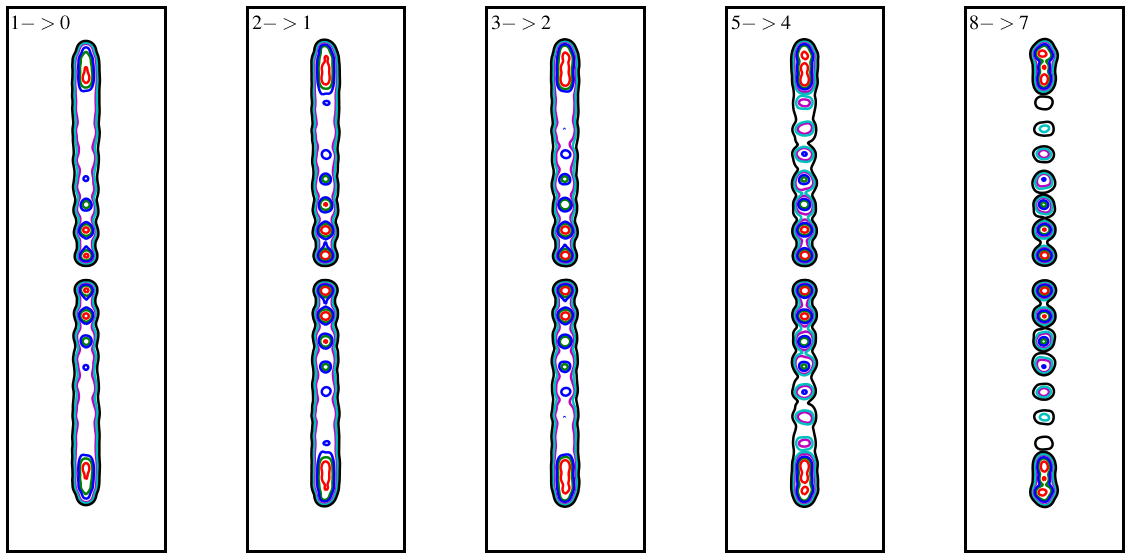
\includegraphics[width=2.\columnwidth]{\figpath/imshkvhcontomaps.png}
 \caption{Contours of SiO emission for different line transitions
   obtained for the run with molecular cooling with $\eta$ = 3 using
   the functional form of the SiO fractional abundance with $\delta <$
   1. The contour colors represent different intensities in Kelvins, i.e,
   30.0({\it red}), 10.0({\it green}), 5.0({\it blue}), 1.0({\it
     magenta}), 0.5({\it cyan}), 0.1({\it black}).} 
\label{fig:ltconts}
\end{figure*}

\cite{Nisini:2007p13128} have shown that the current
plane-parallel shock models fit reasonably well the physical
conditions traced by the SiO emission i.e., temperature $\lesssim$
1000\,K and H$_{2}$ number density $\sim$ 10$^{5}$-10$^{6}$
cm$^{-3}$. They can also fit the observed fractional SiO abundance of
$\sim$ 10$^{-7}$ in these outflows. However, they fail to predict all
the line profiles and in particular their similarities for low and
high excitation lines. Line emission for SiO from our model also traces similar
physical environment. Fig~\ref{fig:Hmolform} shows that regions close
to the internal knot have temperatures up to 1000\,K and molecular
hydrogen density of the order of 10$^{5}$ cm$^{-3}$ about half that of the total
hydrogen density in that region. These regions are where bulk of the
SiO emission is obtained in our models. Additionally, the internal
knots move with velocity of 70-90 km\,s$^{-1}$, indicating a
fractional SiO abundance between 10$^{-6}$ to 10$^{-8}$, depending on the
choice of abundance profile (see fig~\ref{abun}). 
The line profile shapes obtained from this study fit reasonable well with that observed by
\cite{Nisini:2007p13128}, especially for the bullets seen in
L1448. Interestingly, we see in our models, where we relax the plane parallel
approximation, the line profiles are equally broadened for low as well
as high excitation lines. The top panel of fig.~\ref{fig:lineratio} shows spectra for three line
transitions for the reference run but with an angle of inclination,
$\phi$ = 60$^{\circ}$ and convolved with a single dish beam of
15\arcsec. Additionally, the predicted integrated
intensities also lie within a factor of two from the values of L1448 bullets
observed with JCMT and IRAM (Table 2 of \citealt{Nisini:2007p13128}  and
table~\ref{tab:result2} of this work).
%


The variation of integrated single dish emission with upper transition
levels J$_{\rm up}$ for different abundance profiles is shown in the
right panel of fig.~\ref{fig:lineratio}. It is clear, that a emission
obtained using a top hat profile is brighter as compared to one
obtained with a gaussian profile, due to its obvious high estimate of
SiO abundance in regions of interest. However, curves obtained from
both these profiles show a very similar shape of a distinct rise followed by a fall in
integrated emission for higher transitions with a peak in
emission for J$_{\rm up}$ = 3. Similar profiles are also predicted and
used to estimate the physical conditions assuming optically
thin emission from LVG modeling for L1448 and L1157
\cite{Nisini:2007p13128}. However, this usual approach did not give
accurate results for line ratios SiO(8-7)/(5-4) and SiO(5-4)/(2-1)
in case of HH212. Values $\approx$ 1 for both ratios were
only achieved in optically thick LTE regime
\citep{Cabrit:2007p13804, Lee:2008p13697}. 
Similar values are also obtained for molecular outflows from massive
young stellar object IRAS 17233-3606 \cite{Leurini:2013p13165}.
These line ratios from the present
non-LTE radiative transfer model are shown in the bottom left panel of
fig.~\ref{fig:lineratio}. Their values lie very close to unity as
indicated from observations. Further, we have estimated the optical
depth in regions emitting SiO and find them to be optically thick with
an optical depth $\tau \sim 10$. Thus, assuming optically thin SiO emission
from molecular outflows especially from shocked dense knots would
only provide upper limits. In summary, the
shape, ratio and peak intensity of the spectra obtained from our model
fit very well to observed values implying
that SiO emission from our model is tracing the regions with right physical
conditions that are required to emit SiO in gas phase via shocks. 

\begin{figure*}
 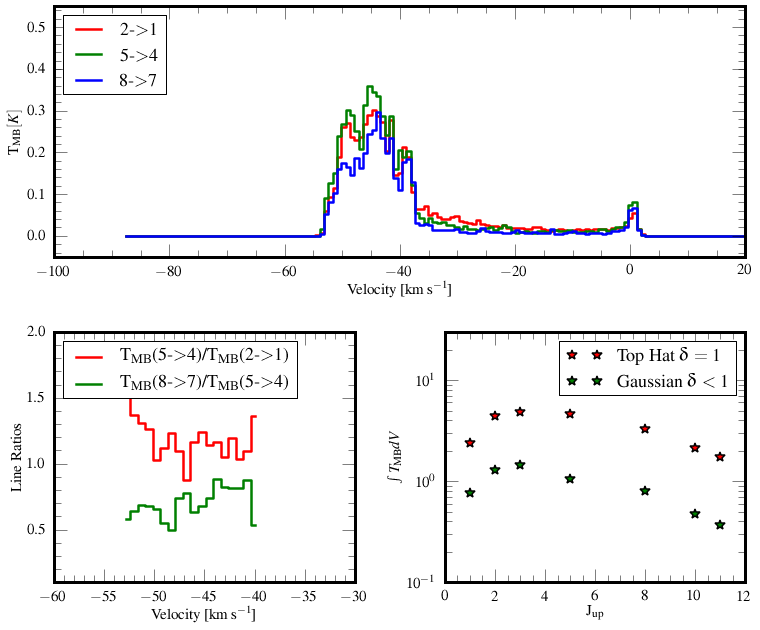
\includegraphics[width=2.\columnwidth]{\figpath/LineRatio_THDeq1.png}
 \caption{{\em{Top}} Line profiles in SiO J = 2-1, 5-4 and 8-7 at one
   the inner knot for the molecular cooling run with $\eta$ = 3 and
   $\beta$ = 10 using top hat abundance profile with $\delta$ = 1. The profiles are
   obtained when the angle of inclination is 60$^{\circ}$ with respect
 to line of sight. {\em{Bottom left}} Line intensity ratios SiO(8-7)/(5-4)
and SiO(5-4)/(2-1), as a function of velocity. {\em{Bottom right}}
Variation of integrated intensity with upper line transition J$_{\rm
  up}$ for two abundance profiles.}
\label{fig:lineratio}
\end{figure*}


\subsection{Slow Component and Grain Chemistry}
%
We have presented a formidable model to explain the EHV component seen
in SiO emission from several young outflows. The reference model
consistently solves for the H$_{2}$ chemistry in presence of
appropriate cooling. The steady state temperature, density and velocities obtained from dynamical
simulation is post-processed to obtain SiO maps, spectra and PV
diagrams. One essential ingredient required for the radiative transfer modeling
is the SiO fractional abundance and its dependence on shock velocity. 
Though 1D models that study the formation of SiO in gas phase from grain-grain and grain-mantle
collisions exsist, their focus is mainly on weaker shocks
\cite{Schilke:1997p14140, Caselli:1997p14853, Gusdorf:2008p13800}. 
The pulsating jet propogation model presented here have shock speeds
reaching upto 100 km\,s$^{-1}$. For simplicity we have used two basic
prescription of SiO abundance profile as a function of shock
velocity. Though the shape of the profile is uncertain the upper and
lower limits used are backed by observational evidences. Ideally for a consistent
depedence of SiO abundance on shock velocity, one would have to also
solve for silicon and SiO chemistry in a manner similar to that of
H$_{2}$. Further by evolving the dynamical simulations with complex
grain chemistry for more than 10$^{4}$ years (time to destroy SiO in
gas phase \cite{Codella:1999p12584}),  one can trace the history of 
SiO in molecular outflows. However, such a numerically expensive model 
with complex chemistry is beyond the scope of this paper.  
%

The model presented in this paper target the very early phase of molecular
outflows i.e., dynamical time scale of 1000 years.
As discussed in sections above, the unqiue combination of pulsating
jet with chemistry and cooling followed by non-LTE radiative transfer
calculations has shown success in fiting the line shapes, integrated intensity and line ratios of SiO
transitions arising from EHV gas. However, the synthetic spectra show
no signatures of slow SiO component that accompanies EHV emission seen
in many outflows. The physical mechanism for the origin of slow SiO component is still a matter
of debate. One of the suggestion is it arises due to slowing down of
shocked gas as they age. The time scale estimated for the shocked gas
to slow down is of the same order of magnitude as the SiO destruction
time scale i.e., 10$^{4}$ years \cite{Codella:1999p12584}. In this
case, we will not be able to see the effect as the dynamical runs do
not evolve beyond 10$^{3}$ years. However, we do see initial 
hints of slowing down of more evolved gas in terms of the velocity
shift of about 5-7 km\,s$^{-1}$ in peak emission between that
coming from the freshly formed internal knots close to the base of the
flow as compared to emission coming from more evolved gas near the
primary bow shock. To ascertain this fact in more details, one would
need to track the primary bow shock for 10$^{4}$ years
using a larger simulation box and possibly with adaptive gridding 
which will be considered for future simulations. Such a long term
evolution will also help to provide a numerical model for the formation of HH objects
which are belived to be slowed down and more evolved form of these
young molecular bullets as suggested by \cite{Norman:1979p14858,
  Hartigan:1987p11178}.
%

Alternative to this evolutinary 




\section{Conclusion}
We are the best in modeling SiO outflows.



%\section*{Acknowledgments}

\bibliographystyle{mn2e}
\bibliography{bibfile}
\label{lastpage}
\end{document}
